\documentclass[twoside]{book}

% Packages required by doxygen
\usepackage{calc}
\usepackage{doxygen}
\usepackage{graphicx}
\usepackage[utf8]{inputenc}
\usepackage{makeidx}
\usepackage{multicol}
\usepackage{multirow}
\usepackage{textcomp}
\usepackage[table]{xcolor}

% Font selection
\usepackage[T1]{fontenc}
\usepackage{mathptmx}
\usepackage[scaled=.90]{helvet}
\usepackage{courier}
\usepackage{amssymb}
\usepackage{sectsty}
\renewcommand{\familydefault}{\sfdefault}
\allsectionsfont{%
  \fontseries{bc}\selectfont%
  \color{darkgray}%
}
\renewcommand{\DoxyLabelFont}{%
  \fontseries{bc}\selectfont%
  \color{darkgray}%
}

% Page & text layout
\usepackage{geometry}
\geometry{%
  a4paper,%
  top=2.5cm,%
  bottom=2.5cm,%
  left=2.5cm,%
  right=2.5cm%
}
\tolerance=750
\hfuzz=15pt
\hbadness=750
\setlength{\emergencystretch}{15pt}
\setlength{\parindent}{0cm}
\setlength{\parskip}{0.2cm}
\makeatletter
\renewcommand{\paragraph}{%
  \@startsection{paragraph}{4}{0ex}{-1.0ex}{1.0ex}{%
    \normalfont\normalsize\bfseries\SS@parafont%
  }%
}
\renewcommand{\subparagraph}{%
  \@startsection{subparagraph}{5}{0ex}{-1.0ex}{1.0ex}{%
    \normalfont\normalsize\bfseries\SS@subparafont%
  }%
}
\makeatother

% Headers & footers
\usepackage{fancyhdr}
\pagestyle{fancyplain}
\fancyhead[LE]{\fancyplain{}{\bfseries\thepage}}
\fancyhead[CE]{\fancyplain{}{}}
\fancyhead[RE]{\fancyplain{}{\bfseries\leftmark}}
\fancyhead[LO]{\fancyplain{}{\bfseries\rightmark}}
\fancyhead[CO]{\fancyplain{}{}}
\fancyhead[RO]{\fancyplain{}{\bfseries\thepage}}
\fancyfoot[LE]{\fancyplain{}{}}
\fancyfoot[CE]{\fancyplain{}{}}
\fancyfoot[RE]{\fancyplain{}{\bfseries\scriptsize Generated on Mon May 2 2016 21\-:20\-:25 for G\-S\-I Project \-: Scheduler by Doxygen }}
\fancyfoot[LO]{\fancyplain{}{\bfseries\scriptsize Generated on Mon May 2 2016 21\-:20\-:25 for G\-S\-I Project \-: Scheduler by Doxygen }}
\fancyfoot[CO]{\fancyplain{}{}}
\fancyfoot[RO]{\fancyplain{}{}}
\renewcommand{\footrulewidth}{0.4pt}
\renewcommand{\chaptermark}[1]{%
  \markboth{#1}{}%
}
\renewcommand{\sectionmark}[1]{%
  \markright{\thesection\ #1}%
}

% Indices & bibliography
\usepackage{natbib}
\usepackage[titles]{tocloft}
\setcounter{tocdepth}{3}
\setcounter{secnumdepth}{5}
\makeindex

% Hyperlinks (required, but should be loaded last)
\usepackage{ifpdf}
\ifpdf
  \usepackage[pdftex,pagebackref=true]{hyperref}
\else
  \usepackage[ps2pdf,pagebackref=true]{hyperref}
\fi
\hypersetup{%
  colorlinks=true,%
  linkcolor=blue,%
  citecolor=blue,%
  unicode%
}

% Custom commands
\newcommand{\clearemptydoublepage}{%
  \newpage{\pagestyle{empty}\cleardoublepage}%
}


%===== C O N T E N T S =====

\begin{document}

% Titlepage & ToC
\hypersetup{pageanchor=false}
\pagenumbering{roman}
\begin{titlepage}
\vspace*{7cm}
\begin{center}%
{\Large G\-S\-I Project \-: Scheduler }\\
\vspace*{1cm}
{\large Generated by Doxygen 1.8.6}\\
\vspace*{0.5cm}
{\small Mon May 2 2016 21:20:25}\\
\end{center}
\end{titlepage}
\clearemptydoublepage
\tableofcontents
\clearemptydoublepage
\pagenumbering{arabic}
\hypersetup{pageanchor=true}

%--- Begin generated contents ---
\chapter{The mainpage documentation}
\label{index}\hypertarget{index}{}\#\-Readme

\subsection*{Documentation}

A special Doxygen documentation has been written for this project. You can read it as html by going to {\ttfamily \$\-P\-R\-O\-J\-E\-C\-T\-\_\-\-R\-O\-O\-T/docs/html/index.html}. You can also build your own documentation using the latex sources at {\ttfamily \$\-P\-R\-O\-J\-E\-C\-T\-\_\-\-R\-O\-O\-T/docs/latex}.

\subsection*{Prerequisite}

In order to compile and run this project you must have installed on your computer the followings \-: C\-Make, Boost, Open\-M\-P \begin{DoxyVerb}# apt-get install cmake libboost-all-dev libopenmpi1.6
\end{DoxyVerb}


\subsection*{Compile sources}

To compile sources, you will have to run the following lines \-: \begin{DoxyVerb}$ mkdir bin && cd bin && cmake .. && make
\end{DoxyVerb}


It will create a folder name 'bin', navigate to it, build the Makefile, and run the Makefile.

\subsection*{Populating}

Use -\/c or --client as argument on the scheduler's executable to start the client. It will populate the queue with your tasks. \begin{DoxyVerb}$ ./Scheduler -c
\end{DoxyVerb}


\subsection*{Scheduling}

Use -\/s or --sequential to start the scheduler in sequential mode. Use -\/p or --parallel to start in parallel. \begin{DoxyVerb}$ ./Scheduler -s
\end{DoxyVerb}


\subsubsection*{Algorithm}

\begin{DoxyVerb}TANT QUE non timeout FAIRE
    -- Une nouvelle tâche arrive
    SI aucun processeur ne peut contenir la tâche
        Attendre qu'un processeur se libère
    SINON
        SI un processeur est vide (pas de tâches en cours)
            lui attribuer automatiquement la tâche.
        SINON
            Récupérer le processeur le moins utilisé
            Lui assigner la tâche
        FINSI
    FINSI
FIN TQ\end{DoxyVerb}
 
\chapter{readme}
\label{md_readme}
\hypertarget{md_readme}{}
\#\-Readme

\subsection*{Documentation}

A special Doxygen documentation has been written for this project. You can read it as html by going to {\ttfamily \$\-P\-R\-O\-J\-E\-C\-T\-\_\-\-R\-O\-O\-T/docs/html/index.html}. You can also build your own documentation using the latex sources at {\ttfamily \$\-P\-R\-O\-J\-E\-C\-T\-\_\-\-R\-O\-O\-T/docs/latex}.

\subsection*{Prerequisite}

In order to compile and run this project you must have installed on your computer the followings \-: C\-Make, Boost, Open\-M\-P \begin{DoxyVerb}# apt-get install cmake libboost-all-dev libopenmpi1.6
\end{DoxyVerb}


\subsection*{Compile sources}

To compile sources, you will have to run the following lines \-: \begin{DoxyVerb}$ mkdir bin && cd bin && cmake .. && make
\end{DoxyVerb}


It will create a folder name 'bin', navigate to it, build the Makefile, and run the Makefile.

\subsection*{Populating}

Use -\/c or --client as argument on the scheduler's executable to start the client. It will populate the queue with your tasks. \begin{DoxyVerb}$ ./Scheduler -c
\end{DoxyVerb}


\subsection*{Scheduling}

Use -\/s or --sequential to start the scheduler in sequential mode. Use -\/p or --parallel to start in parallel. \begin{DoxyVerb}$ ./Scheduler -s
\end{DoxyVerb}


\subsubsection*{Algorithm}

\begin{DoxyVerb}TANT QUE non timeout FAIRE
    -- Une nouvelle tâche arrive
    SI aucun processeur ne peut contenir la tâche
        Attendre qu'un processeur se libère
    SINON
        SI un processeur est vide (pas de tâches en cours)
            lui attribuer automatiquement la tâche.
        SINON
            Récupérer le processeur le moins utilisé
            Lui assigner la tâche
        FINSI
    FINSI
FIN TQ \end{DoxyVerb}
 
\chapter{Hierarchical Index}
\section{Class Hierarchy}
This inheritance list is sorted roughly, but not completely, alphabetically\-:\begin{DoxyCompactList}
\item \contentsline{section}{Client}{\pageref{classClient}}{}
\item \contentsline{section}{Scheduler}{\pageref{classScheduler}}{}
\begin{DoxyCompactList}
\item \contentsline{section}{Parallel\-Scheduler}{\pageref{classParallelScheduler}}{}
\item \contentsline{section}{Sequential\-Scheduler}{\pageref{classSequentialScheduler}}{}
\end{DoxyCompactList}
\item \contentsline{section}{task}{\pageref{structtask}}{}
\end{DoxyCompactList}

\chapter{Class Index}
\section{Class List}
Here are the classes, structs, unions and interfaces with brief descriptions\-:\begin{DoxyCompactList}
\item\contentsline{section}{\hyperlink{classClient}{Client} \\*Class which defines a client sending tasks to a message queue }{\pageref{classClient}}{}
\item\contentsline{section}{\hyperlink{classParallelScheduler}{Parallel\-Scheduler} \\*Class modeling a parallel scheduler }{\pageref{classParallelScheduler}}{}
\item\contentsline{section}{\hyperlink{classScheduler}{Scheduler} \\*This is the base class for the scheduler. Only called by subclass constructor }{\pageref{classScheduler}}{}
\item\contentsline{section}{\hyperlink{classSequentialScheduler}{Sequential\-Scheduler} \\*Class modeling a sequential scheduler }{\pageref{classSequentialScheduler}}{}
\item\contentsline{section}{\hyperlink{structtask}{task} }{\pageref{structtask}}{}
\end{DoxyCompactList}

\chapter{File Index}
\section{File List}
Here is a list of all files with brief descriptions\-:\begin{DoxyCompactList}
\item\contentsline{section}{src/\hyperlink{main_8cpp}{main.\-cpp} \\*Main definition file of the whole program }{\pageref{main_8cpp}}{}
\item\contentsline{section}{src/\hyperlink{main_8h}{main.\-h} \\*Main declaration file of the whole program }{\pageref{main_8h}}{}
\item\contentsline{section}{src/\-Client/\hyperlink{Client_8cpp}{Client.\-cpp} \\*\hyperlink{classClient}{Client} definition class. Send processes to the queue }{\pageref{Client_8cpp}}{}
\item\contentsline{section}{src/\-Client/\hyperlink{Client_8h}{Client.\-h} \\*\hyperlink{classClient}{Client} declaration class }{\pageref{Client_8h}}{}
\item\contentsline{section}{src/\-Scheduler/\hyperlink{ParallelScheduler_8cpp}{Parallel\-Scheduler.\-cpp} \\*Parallel scheduler definition class }{\pageref{ParallelScheduler_8cpp}}{}
\item\contentsline{section}{src/\-Scheduler/\hyperlink{ParallelScheduler_8h}{Parallel\-Scheduler.\-h} \\*Parallel scheduler class declaration }{\pageref{ParallelScheduler_8h}}{}
\item\contentsline{section}{src/\-Scheduler/\hyperlink{Scheduler_8cpp}{Scheduler.\-cpp} \\*\hyperlink{classScheduler}{Scheduler} definition class }{\pageref{Scheduler_8cpp}}{}
\item\contentsline{section}{src/\-Scheduler/\hyperlink{Scheduler_8h}{Scheduler.\-h} \\*\hyperlink{classScheduler}{Scheduler} declaration class }{\pageref{Scheduler_8h}}{}
\item\contentsline{section}{src/\-Scheduler/\hyperlink{SequentialScheduler_8cpp}{Sequential\-Scheduler.\-cpp} \\*Sequential scheduler definition class }{\pageref{SequentialScheduler_8cpp}}{}
\item\contentsline{section}{src/\-Scheduler/\hyperlink{SequentialScheduler_8h}{Sequential\-Scheduler.\-h} \\*Sequential scheduler declaration class }{\pageref{SequentialScheduler_8h}}{}
\item\contentsline{section}{src/util/\hyperlink{flags_8h}{flags.\-h} \\*Flags declaration }{\pageref{flags_8h}}{}
\item\contentsline{section}{src/util/\hyperlink{task_8h}{task.\-h} \\*Task structure declaration }{\pageref{task_8h}}{}
\item\contentsline{section}{src/util/\hyperlink{util_8cpp}{util.\-cpp} \\*Util class definition (functions printing a message) }{\pageref{util_8cpp}}{}
\item\contentsline{section}{src/util/\hyperlink{util_8h}{util.\-h} \\*Util class declaration (functions printing a message) }{\pageref{util_8h}}{}
\end{DoxyCompactList}

\chapter{Class Documentation}
\hypertarget{classClient}{\section{Client Class Reference}
\label{classClient}\index{Client@{Client}}
}


Class which defines a client sending tasks to a message queue.  




{\ttfamily \#include $<$Client.\-h$>$}

\subsection*{Public Member Functions}
\begin{DoxyCompactItemize}
\item 
\hyperlink{classClient_af7faf381e7062b0135ab53c35dbb5542}{Client} (std\-::string)
\begin{DoxyCompactList}\small\item\em \hyperlink{classClient}{Client} class constructor. \end{DoxyCompactList}\item 
\hyperlink{classClient_a840e519ca781888cbd54181572ebe3a7}{$\sim$\-Client} ()
\begin{DoxyCompactList}\small\item\em Default destructor of the class. \end{DoxyCompactList}\item 
void \hyperlink{classClient_a742373e08a80d993d2651b6fff76f5b9}{start} ()
\begin{DoxyCompactList}\small\item\em This function starts the client. \end{DoxyCompactList}\end{DoxyCompactItemize}
\subsection*{Private Member Functions}
\begin{DoxyCompactItemize}
\item 
void \hyperlink{classClient_a8d04b32a55421cf157bc9464bbad74f2}{send\-\_\-one\-\_\-process} ()
\begin{DoxyCompactList}\small\item\em Method to send only one process to the queue. \end{DoxyCompactList}\item 
void \hyperlink{classClient_a4f8c14b12c882c97401b4e3c7965678f}{send\-\_\-several\-\_\-processes} (unsigned)
\begin{DoxyCompactList}\small\item\em Method to send several processes to the queue. \end{DoxyCompactList}\item 
int \hyperlink{classClient_a4a2730dfdf3e84352f79ad85f5306346}{send\-\_\-file\-\_\-processes} ()
\begin{DoxyCompactList}\small\item\em Method to send several processes which are defined in a J\-S\-O\-N file. \end{DoxyCompactList}\end{DoxyCompactItemize}
\subsection*{Private Attributes}
\begin{DoxyCompactItemize}
\item 
std\-::string \hyperlink{classClient_a1585f1f50fcd89691a51031bb11fc36b}{queue\-\_\-name}
\item 
boost\-::interprocess\-::message\-\_\-queue \hyperlink{classClient_ae2045b846aa7287f54e151671a8dd831}{queue}
\end{DoxyCompactItemize}


\subsection{Detailed Description}
Class which defines a client sending tasks to a message queue. 

\subsection{Constructor \& Destructor Documentation}
\hypertarget{classClient_af7faf381e7062b0135ab53c35dbb5542}{\index{Client@{Client}!Client@{Client}}
\index{Client@{Client}!Client@{Client}}
\subsubsection[{Client}]{\setlength{\rightskip}{0pt plus 5cm}Client\-::\-Client (
\begin{DoxyParamCaption}
\item[{std\-::string}]{queue\-\_\-name}
\end{DoxyParamCaption}
)}}\label{classClient_af7faf381e7062b0135ab53c35dbb5542}


\hyperlink{classClient}{Client} class constructor. 


\begin{DoxyParams}{Parameters}
{\em queue\-\_\-name} & the name of the queue \\
\hline
\end{DoxyParams}
\hypertarget{classClient_a840e519ca781888cbd54181572ebe3a7}{\index{Client@{Client}!$\sim$\-Client@{$\sim$\-Client}}
\index{$\sim$\-Client@{$\sim$\-Client}!Client@{Client}}
\subsubsection[{$\sim$\-Client}]{\setlength{\rightskip}{0pt plus 5cm}Client\-::$\sim$\-Client (
\begin{DoxyParamCaption}
{}
\end{DoxyParamCaption}
)}}\label{classClient_a840e519ca781888cbd54181572ebe3a7}


Default destructor of the class. 



\subsection{Member Function Documentation}
\hypertarget{classClient_a4a2730dfdf3e84352f79ad85f5306346}{\index{Client@{Client}!send\-\_\-file\-\_\-processes@{send\-\_\-file\-\_\-processes}}
\index{send\-\_\-file\-\_\-processes@{send\-\_\-file\-\_\-processes}!Client@{Client}}
\subsubsection[{send\-\_\-file\-\_\-processes}]{\setlength{\rightskip}{0pt plus 5cm}int Client\-::send\-\_\-file\-\_\-processes (
\begin{DoxyParamCaption}
{}
\end{DoxyParamCaption}
)\hspace{0.3cm}{\ttfamily [private]}}}\label{classClient_a4a2730dfdf3e84352f79ad85f5306346}


Method to send several processes which are defined in a J\-S\-O\-N file. 

\hypertarget{classClient_a8d04b32a55421cf157bc9464bbad74f2}{\index{Client@{Client}!send\-\_\-one\-\_\-process@{send\-\_\-one\-\_\-process}}
\index{send\-\_\-one\-\_\-process@{send\-\_\-one\-\_\-process}!Client@{Client}}
\subsubsection[{send\-\_\-one\-\_\-process}]{\setlength{\rightskip}{0pt plus 5cm}void Client\-::send\-\_\-one\-\_\-process (
\begin{DoxyParamCaption}
{}
\end{DoxyParamCaption}
)\hspace{0.3cm}{\ttfamily [private]}}}\label{classClient_a8d04b32a55421cf157bc9464bbad74f2}


Method to send only one process to the queue. 

\hypertarget{classClient_a4f8c14b12c882c97401b4e3c7965678f}{\index{Client@{Client}!send\-\_\-several\-\_\-processes@{send\-\_\-several\-\_\-processes}}
\index{send\-\_\-several\-\_\-processes@{send\-\_\-several\-\_\-processes}!Client@{Client}}
\subsubsection[{send\-\_\-several\-\_\-processes}]{\setlength{\rightskip}{0pt plus 5cm}void Client\-::send\-\_\-several\-\_\-processes (
\begin{DoxyParamCaption}
\item[{unsigned}]{nb\-\_\-processes}
\end{DoxyParamCaption}
)\hspace{0.3cm}{\ttfamily [private]}}}\label{classClient_a4f8c14b12c882c97401b4e3c7965678f}


Method to send several processes to the queue. 


\begin{DoxyParams}{Parameters}
{\em Number} & of processes to send \\
\hline
\end{DoxyParams}
\hypertarget{classClient_a742373e08a80d993d2651b6fff76f5b9}{\index{Client@{Client}!start@{start}}
\index{start@{start}!Client@{Client}}
\subsubsection[{start}]{\setlength{\rightskip}{0pt plus 5cm}void Client\-::start (
\begin{DoxyParamCaption}
{}
\end{DoxyParamCaption}
)}}\label{classClient_a742373e08a80d993d2651b6fff76f5b9}


This function starts the client. 



\subsection{Member Data Documentation}
\hypertarget{classClient_ae2045b846aa7287f54e151671a8dd831}{\index{Client@{Client}!queue@{queue}}
\index{queue@{queue}!Client@{Client}}
\subsubsection[{queue}]{\setlength{\rightskip}{0pt plus 5cm}boost\-::interprocess\-::message\-\_\-queue Client\-::queue\hspace{0.3cm}{\ttfamily [private]}}}\label{classClient_ae2045b846aa7287f54e151671a8dd831}
Queue \hypertarget{classClient_a1585f1f50fcd89691a51031bb11fc36b}{\index{Client@{Client}!queue\-\_\-name@{queue\-\_\-name}}
\index{queue\-\_\-name@{queue\-\_\-name}!Client@{Client}}
\subsubsection[{queue\-\_\-name}]{\setlength{\rightskip}{0pt plus 5cm}std\-::string Client\-::queue\-\_\-name\hspace{0.3cm}{\ttfamily [private]}}}\label{classClient_a1585f1f50fcd89691a51031bb11fc36b}
Queue\-\_\-name 

The documentation for this class was generated from the following files\-:\begin{DoxyCompactItemize}
\item 
src/\-Client/\hyperlink{Client_8h}{Client.\-h}\item 
src/\-Client/\hyperlink{Client_8cpp}{Client.\-cpp}\end{DoxyCompactItemize}

\hypertarget{classParallelScheduler}{\section{Parallel\-Scheduler Class Reference}
\label{classParallelScheduler}\index{Parallel\-Scheduler@{Parallel\-Scheduler}}
}


Class modeling a parallel scheduler.  




{\ttfamily \#include $<$Parallel\-Scheduler.\-h$>$}

Inheritance diagram for Parallel\-Scheduler\-:\begin{figure}[H]
\begin{center}
\leavevmode
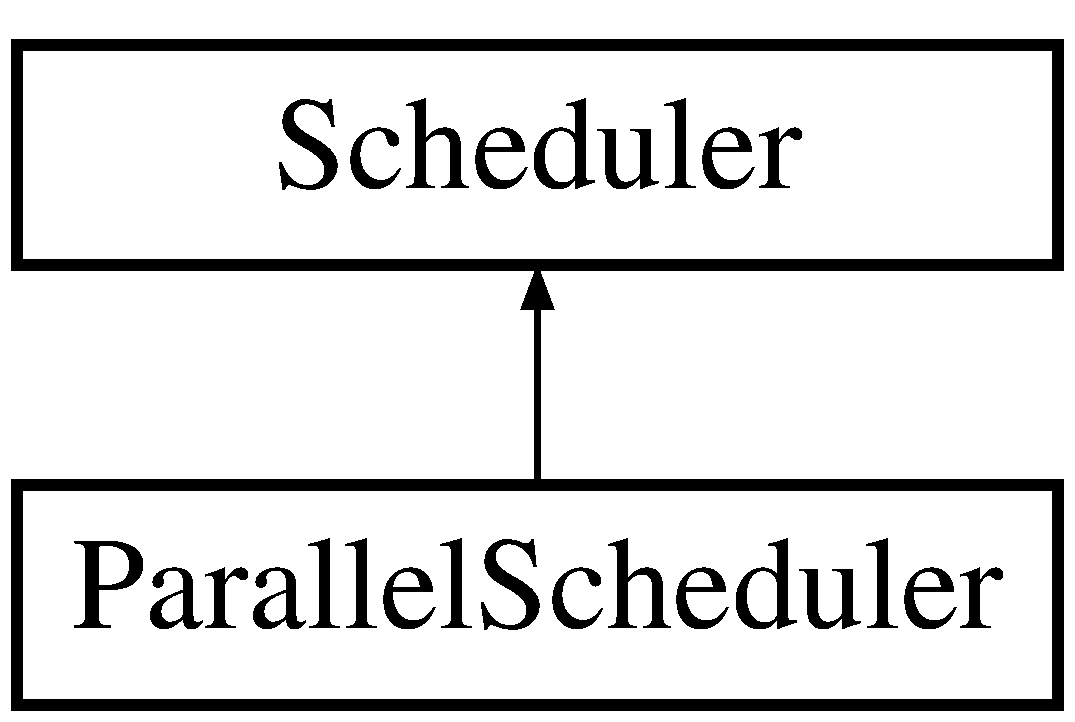
\includegraphics[height=2.000000cm]{classParallelScheduler}
\end{center}
\end{figure}
\subsection*{Public Member Functions}
\begin{DoxyCompactItemize}
\item 
\hyperlink{classParallelScheduler_a11e91f323808008a8a35961aa84211bf}{Parallel\-Scheduler} (std\-::string, std\-::string, int)
\begin{DoxyCompactList}\small\item\em Parallel scheduler class constructor. \end{DoxyCompactList}\item 
virtual \hyperlink{classParallelScheduler_a995351f4556a464e6c4a78e01cea583c}{$\sim$\-Parallel\-Scheduler} ()
\begin{DoxyCompactList}\small\item\em Default parallel scheduler class destructor. \end{DoxyCompactList}\item 
virtual void \hyperlink{classParallelScheduler_aef0d5f1091857170434687897d19843e}{start} ()
\begin{DoxyCompactList}\small\item\em This method starts the scheduler in parallel mode. \end{DoxyCompactList}\end{DoxyCompactItemize}
\subsection*{Private Member Functions}
\begin{DoxyCompactItemize}
\item 
int \hyperlink{classParallelScheduler_a3a3bd8e72a7dbc83986cf31918569fd3}{get\-\_\-unloaded\-\_\-core} (const std\-::vector$<$ double $>$ \&)
\begin{DoxyCompactList}\small\item\em Method looking for an unloaded core and returning its index. \end{DoxyCompactList}\item 
int \hyperlink{classParallelScheduler_ad58ae6d78d6920e548d7c6c956fa3caa}{get\-\_\-less\-\_\-loaded\-\_\-core} (const std\-::vector$<$ double $>$ \&)
\begin{DoxyCompactList}\small\item\em Method looking for the less loaded core. \end{DoxyCompactList}\item 
bool \hyperlink{classParallelScheduler_af52a8e359a4134fec49db090781caf8b}{exist\-\_\-suitable\-\_\-core} (const std\-::vector$<$ double $>$ \&, double)
\begin{DoxyCompactList}\small\item\em Method looking for a core which can handle the task. \end{DoxyCompactList}\item 
void \hyperlink{classParallelScheduler_a7925556ff7ab1b4746a72709b24f157e}{get\-\_\-cores\-\_\-load} (const \hyperlink{ParallelScheduler_8h_ac7eb1fba35a2c780a99ff2d3df789884}{Vector\-Tasks} \&, std\-::vector$<$ double $>$ \&)
\begin{DoxyCompactList}\small\item\em Method retrieving the load of each core and filling cores\-\_\-load with the data. \end{DoxyCompactList}\item 
int \hyperlink{classParallelScheduler_ad71e8b952aee7b123c612540564fa090}{get\-\_\-core\-\_\-to\-\_\-assign} (const \hyperlink{ParallelScheduler_8h_ac7eb1fba35a2c780a99ff2d3df789884}{Vector\-Tasks} \&, double)
\begin{DoxyCompactList}\small\item\em Main method looking for a core that can handle the task. \end{DoxyCompactList}\end{DoxyCompactItemize}
\subsection*{Private Attributes}
\begin{DoxyCompactItemize}
\item 
std\-::string \hyperlink{classParallelScheduler_a5cd72cd536a5183e04b922fa2eb7235e}{filename}
\item 
std\-::string \hyperlink{classParallelScheduler_a76e34b4f290c1c4ad68ea3b5429c0ba4}{queue\-\_\-name}
\end{DoxyCompactItemize}
\subsection*{Additional Inherited Members}


\subsection{Detailed Description}
Class modeling a parallel scheduler. 

\subsection{Constructor \& Destructor Documentation}
\hypertarget{classParallelScheduler_a11e91f323808008a8a35961aa84211bf}{\index{Parallel\-Scheduler@{Parallel\-Scheduler}!Parallel\-Scheduler@{Parallel\-Scheduler}}
\index{Parallel\-Scheduler@{Parallel\-Scheduler}!ParallelScheduler@{Parallel\-Scheduler}}
\subsubsection[{Parallel\-Scheduler}]{\setlength{\rightskip}{0pt plus 5cm}Parallel\-Scheduler\-::\-Parallel\-Scheduler (
\begin{DoxyParamCaption}
\item[{std\-::string}]{queue\-\_\-name, }
\item[{std\-::string}]{filename, }
\item[{int}]{ncores}
\end{DoxyParamCaption}
)}}\label{classParallelScheduler_a11e91f323808008a8a35961aa84211bf}


Parallel scheduler class constructor. 


\begin{DoxyParams}{Parameters}
{\em queue\-\_\-name} & the name of the message queue \\
\hline
{\em filename} & name of the file which will be opened as the stream file\-\_\-logs \\
\hline
{\em ncores} & number of cores available for the scheduler \\
\hline
\end{DoxyParams}
\hypertarget{classParallelScheduler_a995351f4556a464e6c4a78e01cea583c}{\index{Parallel\-Scheduler@{Parallel\-Scheduler}!$\sim$\-Parallel\-Scheduler@{$\sim$\-Parallel\-Scheduler}}
\index{$\sim$\-Parallel\-Scheduler@{$\sim$\-Parallel\-Scheduler}!ParallelScheduler@{Parallel\-Scheduler}}
\subsubsection[{$\sim$\-Parallel\-Scheduler}]{\setlength{\rightskip}{0pt plus 5cm}Parallel\-Scheduler\-::$\sim$\-Parallel\-Scheduler (
\begin{DoxyParamCaption}
{}
\end{DoxyParamCaption}
)\hspace{0.3cm}{\ttfamily [virtual]}}}\label{classParallelScheduler_a995351f4556a464e6c4a78e01cea583c}


Default parallel scheduler class destructor. 



\subsection{Member Function Documentation}
\hypertarget{classParallelScheduler_af52a8e359a4134fec49db090781caf8b}{\index{Parallel\-Scheduler@{Parallel\-Scheduler}!exist\-\_\-suitable\-\_\-core@{exist\-\_\-suitable\-\_\-core}}
\index{exist\-\_\-suitable\-\_\-core@{exist\-\_\-suitable\-\_\-core}!ParallelScheduler@{Parallel\-Scheduler}}
\subsubsection[{exist\-\_\-suitable\-\_\-core}]{\setlength{\rightskip}{0pt plus 5cm}bool Parallel\-Scheduler\-::exist\-\_\-suitable\-\_\-core (
\begin{DoxyParamCaption}
\item[{const std\-::vector$<$ double $>$ \&}]{cores\-\_\-load, }
\item[{double}]{task\-\_\-load}
\end{DoxyParamCaption}
)\hspace{0.3cm}{\ttfamily [private]}}}\label{classParallelScheduler_af52a8e359a4134fec49db090781caf8b}


Method looking for a core which can handle the task. 


\begin{DoxyParams}{Parameters}
{\em cores\-\_\-load} & vector containing the load of each core \\
\hline
{\em task\-\_\-load} & the task's load \\
\hline
\end{DoxyParams}
\begin{DoxyReturn}{Returns}
true if a core exists, false otherwise 
\end{DoxyReturn}
\hypertarget{classParallelScheduler_ad71e8b952aee7b123c612540564fa090}{\index{Parallel\-Scheduler@{Parallel\-Scheduler}!get\-\_\-core\-\_\-to\-\_\-assign@{get\-\_\-core\-\_\-to\-\_\-assign}}
\index{get\-\_\-core\-\_\-to\-\_\-assign@{get\-\_\-core\-\_\-to\-\_\-assign}!ParallelScheduler@{Parallel\-Scheduler}}
\subsubsection[{get\-\_\-core\-\_\-to\-\_\-assign}]{\setlength{\rightskip}{0pt plus 5cm}int Parallel\-Scheduler\-::get\-\_\-core\-\_\-to\-\_\-assign (
\begin{DoxyParamCaption}
\item[{const {\bf Vector\-Tasks} \&}]{process\-\_\-list, }
\item[{double}]{task\-\_\-load}
\end{DoxyParamCaption}
)\hspace{0.3cm}{\ttfamily [private]}}}\label{classParallelScheduler_ad71e8b952aee7b123c612540564fa090}


Main method looking for a core that can handle the task. 


\begin{DoxyParams}{Parameters}
{\em process\-\_\-list} & vector containing the tasks that which are assigned to a core \\
\hline
{\em task\-\_\-load} & the load of the task \\
\hline
\end{DoxyParams}
\begin{DoxyReturn}{Returns}
index of the core if there's one, -\/1 otherwise 
\end{DoxyReturn}
\hypertarget{classParallelScheduler_a7925556ff7ab1b4746a72709b24f157e}{\index{Parallel\-Scheduler@{Parallel\-Scheduler}!get\-\_\-cores\-\_\-load@{get\-\_\-cores\-\_\-load}}
\index{get\-\_\-cores\-\_\-load@{get\-\_\-cores\-\_\-load}!ParallelScheduler@{Parallel\-Scheduler}}
\subsubsection[{get\-\_\-cores\-\_\-load}]{\setlength{\rightskip}{0pt plus 5cm}void Parallel\-Scheduler\-::get\-\_\-cores\-\_\-load (
\begin{DoxyParamCaption}
\item[{const {\bf Vector\-Tasks} \&}]{process\-\_\-list, }
\item[{std\-::vector$<$ double $>$ \&}]{cores\-\_\-load}
\end{DoxyParamCaption}
)\hspace{0.3cm}{\ttfamily [private]}}}\label{classParallelScheduler_a7925556ff7ab1b4746a72709b24f157e}


Method retrieving the load of each core and filling cores\-\_\-load with the data. 


\begin{DoxyParams}{Parameters}
{\em process\-\_\-list} & vector containing the tasks which are assigned to a core \\
\hline
{\em cores\-\_\-load} & vector containing the load of each core \\
\hline
\end{DoxyParams}
\hypertarget{classParallelScheduler_ad58ae6d78d6920e548d7c6c956fa3caa}{\index{Parallel\-Scheduler@{Parallel\-Scheduler}!get\-\_\-less\-\_\-loaded\-\_\-core@{get\-\_\-less\-\_\-loaded\-\_\-core}}
\index{get\-\_\-less\-\_\-loaded\-\_\-core@{get\-\_\-less\-\_\-loaded\-\_\-core}!ParallelScheduler@{Parallel\-Scheduler}}
\subsubsection[{get\-\_\-less\-\_\-loaded\-\_\-core}]{\setlength{\rightskip}{0pt plus 5cm}int Parallel\-Scheduler\-::get\-\_\-less\-\_\-loaded\-\_\-core (
\begin{DoxyParamCaption}
\item[{const std\-::vector$<$ double $>$ \&}]{cores\-\_\-load}
\end{DoxyParamCaption}
)\hspace{0.3cm}{\ttfamily [private]}}}\label{classParallelScheduler_ad58ae6d78d6920e548d7c6c956fa3caa}


Method looking for the less loaded core. 


\begin{DoxyParams}{Parameters}
{\em cores\-\_\-load} & vector containing the load of each core \\
\hline
\end{DoxyParams}
\begin{DoxyReturn}{Returns}
index of the less loaded core 
\end{DoxyReturn}
\hypertarget{classParallelScheduler_a3a3bd8e72a7dbc83986cf31918569fd3}{\index{Parallel\-Scheduler@{Parallel\-Scheduler}!get\-\_\-unloaded\-\_\-core@{get\-\_\-unloaded\-\_\-core}}
\index{get\-\_\-unloaded\-\_\-core@{get\-\_\-unloaded\-\_\-core}!ParallelScheduler@{Parallel\-Scheduler}}
\subsubsection[{get\-\_\-unloaded\-\_\-core}]{\setlength{\rightskip}{0pt plus 5cm}int Parallel\-Scheduler\-::get\-\_\-unloaded\-\_\-core (
\begin{DoxyParamCaption}
\item[{const std\-::vector$<$ double $>$ \&}]{cores\-\_\-load}
\end{DoxyParamCaption}
)\hspace{0.3cm}{\ttfamily [private]}}}\label{classParallelScheduler_a3a3bd8e72a7dbc83986cf31918569fd3}


Method looking for an unloaded core and returning its index. 


\begin{DoxyParams}{Parameters}
{\em cores\-\_\-load} & vector containing the load of each core \\
\hline
\end{DoxyParams}
\begin{DoxyReturn}{Returns}
index of the unloaded core or -\/1 if no core 
\end{DoxyReturn}
\hypertarget{classParallelScheduler_aef0d5f1091857170434687897d19843e}{\index{Parallel\-Scheduler@{Parallel\-Scheduler}!start@{start}}
\index{start@{start}!ParallelScheduler@{Parallel\-Scheduler}}
\subsubsection[{start}]{\setlength{\rightskip}{0pt plus 5cm}void Parallel\-Scheduler\-::start (
\begin{DoxyParamCaption}
{}
\end{DoxyParamCaption}
)\hspace{0.3cm}{\ttfamily [virtual]}}}\label{classParallelScheduler_aef0d5f1091857170434687897d19843e}


This method starts the scheduler in parallel mode. 



Implements \hyperlink{classScheduler_aaa8fed2f8fab3a5c0e5d1d462915e415}{Scheduler}.



\subsection{Member Data Documentation}
\hypertarget{classParallelScheduler_a5cd72cd536a5183e04b922fa2eb7235e}{\index{Parallel\-Scheduler@{Parallel\-Scheduler}!filename@{filename}}
\index{filename@{filename}!ParallelScheduler@{Parallel\-Scheduler}}
\subsubsection[{filename}]{\setlength{\rightskip}{0pt plus 5cm}std\-::string Parallel\-Scheduler\-::filename\hspace{0.3cm}{\ttfamily [private]}}}\label{classParallelScheduler_a5cd72cd536a5183e04b922fa2eb7235e}
ame of the file which will be opened as the stream file\-\_\-logs \hypertarget{classParallelScheduler_a76e34b4f290c1c4ad68ea3b5429c0ba4}{\index{Parallel\-Scheduler@{Parallel\-Scheduler}!queue\-\_\-name@{queue\-\_\-name}}
\index{queue\-\_\-name@{queue\-\_\-name}!ParallelScheduler@{Parallel\-Scheduler}}
\subsubsection[{queue\-\_\-name}]{\setlength{\rightskip}{0pt plus 5cm}std\-::string Parallel\-Scheduler\-::queue\-\_\-name\hspace{0.3cm}{\ttfamily [private]}}}\label{classParallelScheduler_a76e34b4f290c1c4ad68ea3b5429c0ba4}
Name of the queue 

The documentation for this class was generated from the following files\-:\begin{DoxyCompactItemize}
\item 
src/\-Scheduler/\hyperlink{ParallelScheduler_8h}{Parallel\-Scheduler.\-h}\item 
src/\-Scheduler/\hyperlink{ParallelScheduler_8cpp}{Parallel\-Scheduler.\-cpp}\end{DoxyCompactItemize}

\hypertarget{classScheduler}{\section{Scheduler Class Reference}
\label{classScheduler}\index{Scheduler@{Scheduler}}
}


This is the base class for the scheduler. Only called by subclass constructor.  




{\ttfamily \#include $<$Scheduler.\-h$>$}

Inheritance diagram for Scheduler\-:\begin{figure}[H]
\begin{center}
\leavevmode
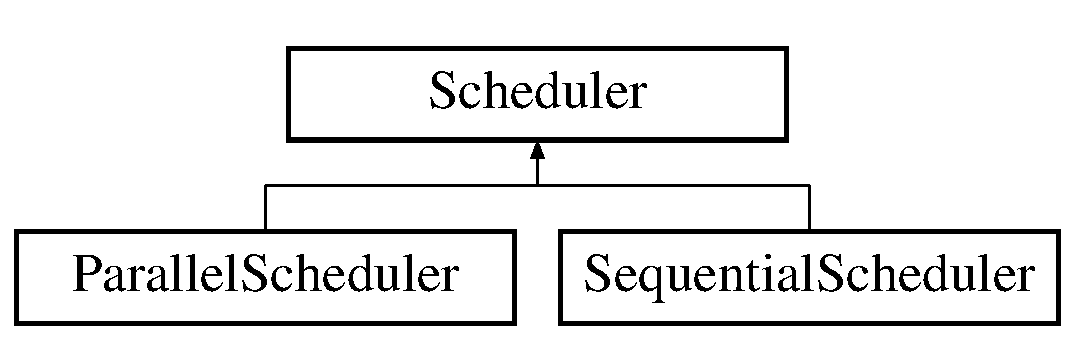
\includegraphics[height=2.000000cm]{classScheduler}
\end{center}
\end{figure}
\subsection*{Public Member Functions}
\begin{DoxyCompactItemize}
\item 
\hyperlink{classScheduler_abff3c6b4c4c7823bdf4b61f2116e1c13}{Scheduler} (std\-::string, int)
\begin{DoxyCompactList}\small\item\em \hyperlink{classScheduler}{Scheduler} class constructor. \end{DoxyCompactList}\item 
virtual \hyperlink{classScheduler_afc8187779b46f64039d3ffa58f0dbe51}{$\sim$\-Scheduler} ()
\begin{DoxyCompactList}\small\item\em Default scheduler destructor. \end{DoxyCompactList}\end{DoxyCompactItemize}
\subsection*{Protected Member Functions}
\begin{DoxyCompactItemize}
\item 
void \hyperlink{classScheduler_a1befb7a203a0e28730e5aa6489bc2a44}{init\-Cores} ()
\begin{DoxyCompactList}\small\item\em Method initializing each core's load to 0. \end{DoxyCompactList}\item 
virtual void \hyperlink{classScheduler_aaa8fed2f8fab3a5c0e5d1d462915e415}{start} ()=0
\begin{DoxyCompactList}\small\item\em Pure virtual method. Will be implemented by the subclasses and never called. \end{DoxyCompactList}\end{DoxyCompactItemize}
\subsection*{Protected Attributes}
\begin{DoxyCompactItemize}
\item 
std\-::fstream \hyperlink{classScheduler_aaa404121f2a46a4012fc6b11374dae29}{file\-\_\-logs}
\item 
std\-::vector$<$ double $>$ \hyperlink{classScheduler_a6f6825fef1ef0a243ebd42751f2186f9}{cores\-\_\-load}
\end{DoxyCompactItemize}
\subsection*{Private Attributes}
\begin{DoxyCompactItemize}
\item 
int \hyperlink{classScheduler_ac2ae53ef390e5372fdfb9c850f91d0c7}{ncores}
\end{DoxyCompactItemize}


\subsection{Detailed Description}
This is the base class for the scheduler. Only called by subclass constructor. 

\subsection{Constructor \& Destructor Documentation}
\hypertarget{classScheduler_abff3c6b4c4c7823bdf4b61f2116e1c13}{\index{Scheduler@{Scheduler}!Scheduler@{Scheduler}}
\index{Scheduler@{Scheduler}!Scheduler@{Scheduler}}
\subsubsection[{Scheduler}]{\setlength{\rightskip}{0pt plus 5cm}Scheduler\-::\-Scheduler (
\begin{DoxyParamCaption}
\item[{std\-::string}]{filename, }
\item[{int}]{ncores}
\end{DoxyParamCaption}
)}}\label{classScheduler_abff3c6b4c4c7823bdf4b61f2116e1c13}


\hyperlink{classScheduler}{Scheduler} class constructor. 


\begin{DoxyParams}{Parameters}
{\em filename} & name of the file which will be opened as the stream file\-\_\-logs \\
\hline
{\em ncores} & number of cores available for the scheduler \\
\hline
\end{DoxyParams}
\hypertarget{classScheduler_afc8187779b46f64039d3ffa58f0dbe51}{\index{Scheduler@{Scheduler}!$\sim$\-Scheduler@{$\sim$\-Scheduler}}
\index{$\sim$\-Scheduler@{$\sim$\-Scheduler}!Scheduler@{Scheduler}}
\subsubsection[{$\sim$\-Scheduler}]{\setlength{\rightskip}{0pt plus 5cm}Scheduler\-::$\sim$\-Scheduler (
\begin{DoxyParamCaption}
{}
\end{DoxyParamCaption}
)\hspace{0.3cm}{\ttfamily [virtual]}}}\label{classScheduler_afc8187779b46f64039d3ffa58f0dbe51}


Default scheduler destructor. 



\subsection{Member Function Documentation}
\hypertarget{classScheduler_a1befb7a203a0e28730e5aa6489bc2a44}{\index{Scheduler@{Scheduler}!init\-Cores@{init\-Cores}}
\index{init\-Cores@{init\-Cores}!Scheduler@{Scheduler}}
\subsubsection[{init\-Cores}]{\setlength{\rightskip}{0pt plus 5cm}void Scheduler\-::init\-Cores (
\begin{DoxyParamCaption}
{}
\end{DoxyParamCaption}
)\hspace{0.3cm}{\ttfamily [protected]}}}\label{classScheduler_a1befb7a203a0e28730e5aa6489bc2a44}


Method initializing each core's load to 0. 

\hypertarget{classScheduler_aaa8fed2f8fab3a5c0e5d1d462915e415}{\index{Scheduler@{Scheduler}!start@{start}}
\index{start@{start}!Scheduler@{Scheduler}}
\subsubsection[{start}]{\setlength{\rightskip}{0pt plus 5cm}virtual void Scheduler\-::start (
\begin{DoxyParamCaption}
{}
\end{DoxyParamCaption}
)\hspace{0.3cm}{\ttfamily [protected]}, {\ttfamily [pure virtual]}}}\label{classScheduler_aaa8fed2f8fab3a5c0e5d1d462915e415}


Pure virtual method. Will be implemented by the subclasses and never called. 



Implemented in \hyperlink{classSequentialScheduler_a9603767b779a4612f02ac85bc4c49bf6}{Sequential\-Scheduler}, and \hyperlink{classParallelScheduler_aef0d5f1091857170434687897d19843e}{Parallel\-Scheduler}.



\subsection{Member Data Documentation}
\hypertarget{classScheduler_a6f6825fef1ef0a243ebd42751f2186f9}{\index{Scheduler@{Scheduler}!cores\-\_\-load@{cores\-\_\-load}}
\index{cores\-\_\-load@{cores\-\_\-load}!Scheduler@{Scheduler}}
\subsubsection[{cores\-\_\-load}]{\setlength{\rightskip}{0pt plus 5cm}std\-::vector$<$double$>$ Scheduler\-::cores\-\_\-load\hspace{0.3cm}{\ttfamily [protected]}}}\label{classScheduler_a6f6825fef1ef0a243ebd42751f2186f9}
vector containing each core's load \hypertarget{classScheduler_aaa404121f2a46a4012fc6b11374dae29}{\index{Scheduler@{Scheduler}!file\-\_\-logs@{file\-\_\-logs}}
\index{file\-\_\-logs@{file\-\_\-logs}!Scheduler@{Scheduler}}
\subsubsection[{file\-\_\-logs}]{\setlength{\rightskip}{0pt plus 5cm}std\-::fstream Scheduler\-::file\-\_\-logs\hspace{0.3cm}{\ttfamily [protected]}}}\label{classScheduler_aaa404121f2a46a4012fc6b11374dae29}
Stream to a local file. Used to write the scheduler's logs \hypertarget{classScheduler_ac2ae53ef390e5372fdfb9c850f91d0c7}{\index{Scheduler@{Scheduler}!ncores@{ncores}}
\index{ncores@{ncores}!Scheduler@{Scheduler}}
\subsubsection[{ncores}]{\setlength{\rightskip}{0pt plus 5cm}int Scheduler\-::ncores\hspace{0.3cm}{\ttfamily [private]}}}\label{classScheduler_ac2ae53ef390e5372fdfb9c850f91d0c7}
Number of cores available for the scheduler 

The documentation for this class was generated from the following files\-:\begin{DoxyCompactItemize}
\item 
src/\-Scheduler/\hyperlink{Scheduler_8h}{Scheduler.\-h}\item 
src/\-Scheduler/\hyperlink{Scheduler_8cpp}{Scheduler.\-cpp}\end{DoxyCompactItemize}

\hypertarget{classSequentialScheduler}{\section{Sequential\-Scheduler Class Reference}
\label{classSequentialScheduler}\index{Sequential\-Scheduler@{Sequential\-Scheduler}}
}


Class modeling a sequential scheduler.  




{\ttfamily \#include $<$Sequential\-Scheduler.\-h$>$}

Inheritance diagram for Sequential\-Scheduler\-:\begin{figure}[H]
\begin{center}
\leavevmode
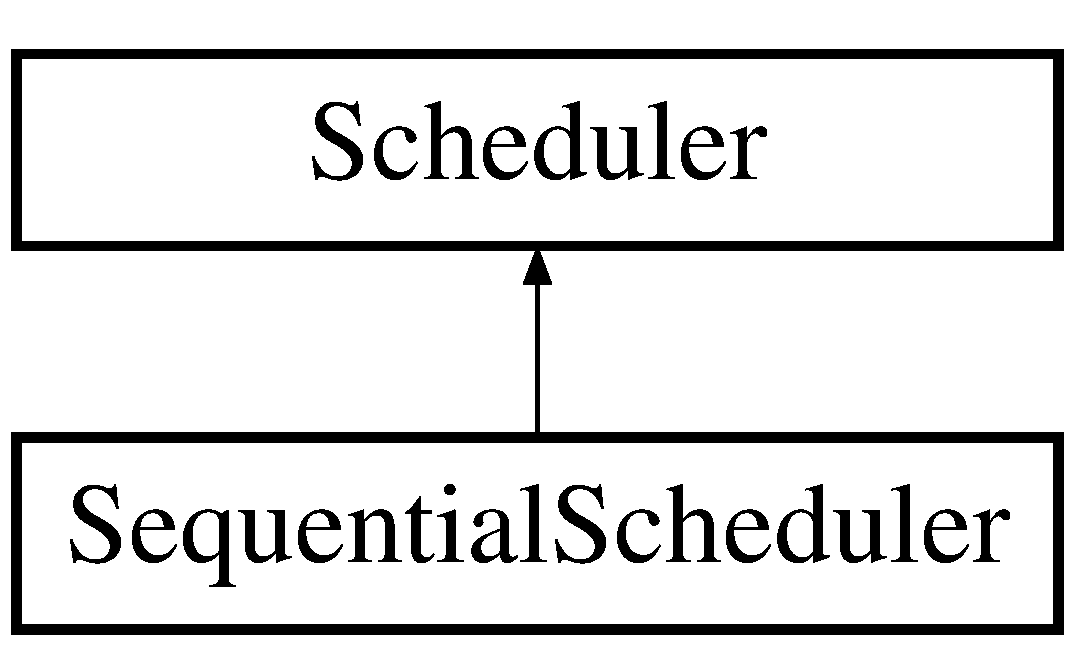
\includegraphics[height=2.000000cm]{classSequentialScheduler}
\end{center}
\end{figure}
\subsection*{Public Member Functions}
\begin{DoxyCompactItemize}
\item 
\hyperlink{classSequentialScheduler_a4c04f1691f53c150a1fe2a2be5a92bed}{Sequential\-Scheduler} (const std\-::string \&, const std\-::string \&, int)
\begin{DoxyCompactList}\small\item\em Sequential scheduler class constructor. \end{DoxyCompactList}\item 
virtual \hyperlink{classSequentialScheduler_a4603b4f03aba99b87a80d75f68dbd746}{$\sim$\-Sequential\-Scheduler} ()
\begin{DoxyCompactList}\small\item\em Default sequential scheduler class destructor. \end{DoxyCompactList}\item 
virtual void \hyperlink{classSequentialScheduler_a9603767b779a4612f02ac85bc4c49bf6}{start} ()
\begin{DoxyCompactList}\small\item\em This method starts the scheduler in sequential mode. \end{DoxyCompactList}\end{DoxyCompactItemize}
\subsection*{Private Member Functions}
\begin{DoxyCompactItemize}
\item 
int \hyperlink{classSequentialScheduler_ae8af6ea6af9b34144e657e208e5bf23e}{get\-\_\-unloaded\-\_\-core} (const std\-::vector$<$ double $>$ \&)
\begin{DoxyCompactList}\small\item\em Method looking for an unloaded core and returning its index. \end{DoxyCompactList}\item 
int \hyperlink{classSequentialScheduler_a7731305cd82efe8c55af85d654996d90}{get\-\_\-less\-\_\-loaded\-\_\-core} (const std\-::vector$<$ double $>$ \&)
\begin{DoxyCompactList}\small\item\em Method looking for the less loaded core. \end{DoxyCompactList}\item 
bool \hyperlink{classSequentialScheduler_a4155dae41da7b17bee2e784e03ecad8f}{exist\-\_\-suitable\-\_\-core} (const std\-::vector$<$ double $>$ \&, double)
\begin{DoxyCompactList}\small\item\em Method looking for a core which can handle the task. \end{DoxyCompactList}\item 
void \hyperlink{classSequentialScheduler_a76d17fb75bdd0cee7284086581a18515}{get\-\_\-cores\-\_\-load} (const \hyperlink{ParallelScheduler_8h_ac7eb1fba35a2c780a99ff2d3df789884}{Vector\-Tasks} \&, std\-::vector$<$ double $>$ \&)
\begin{DoxyCompactList}\small\item\em Method retrieving the load of each core and filling cores\-\_\-load with the data. \end{DoxyCompactList}\item 
int \hyperlink{classSequentialScheduler_af4c223d08734e1daa294ae19d74ca4f1}{get\-\_\-core\-\_\-to\-\_\-assign} (const \hyperlink{ParallelScheduler_8h_ac7eb1fba35a2c780a99ff2d3df789884}{Vector\-Tasks} \&, double)
\begin{DoxyCompactList}\small\item\em Main method looking for a core that can handle the task. \end{DoxyCompactList}\end{DoxyCompactItemize}
\subsection*{Private Attributes}
\begin{DoxyCompactItemize}
\item 
std\-::string \hyperlink{classSequentialScheduler_a86b32eaf91dbc706879c43194142d554}{filename}
\item 
std\-::string \hyperlink{classSequentialScheduler_a2bb2fec195ae97c733509221cf6f293f}{queue\-\_\-name}
\end{DoxyCompactItemize}
\subsection*{Additional Inherited Members}


\subsection{Detailed Description}
Class modeling a sequential scheduler. 

\subsection{Constructor \& Destructor Documentation}
\hypertarget{classSequentialScheduler_a4c04f1691f53c150a1fe2a2be5a92bed}{\index{Sequential\-Scheduler@{Sequential\-Scheduler}!Sequential\-Scheduler@{Sequential\-Scheduler}}
\index{Sequential\-Scheduler@{Sequential\-Scheduler}!SequentialScheduler@{Sequential\-Scheduler}}
\subsubsection[{Sequential\-Scheduler}]{\setlength{\rightskip}{0pt plus 5cm}Sequential\-Scheduler\-::\-Sequential\-Scheduler (
\begin{DoxyParamCaption}
\item[{const std\-::string \&}]{queue\-\_\-name, }
\item[{const std\-::string \&}]{filename, }
\item[{int}]{ncores}
\end{DoxyParamCaption}
)}}\label{classSequentialScheduler_a4c04f1691f53c150a1fe2a2be5a92bed}


Sequential scheduler class constructor. 


\begin{DoxyParams}{Parameters}
{\em queue\-\_\-name} & the name of the message queue \\
\hline
{\em filename} & name of the file which will be opened as the stream file\-\_\-logs \\
\hline
{\em ncores} & number of cores available for the scheduler \\
\hline
\end{DoxyParams}
\hypertarget{classSequentialScheduler_a4603b4f03aba99b87a80d75f68dbd746}{\index{Sequential\-Scheduler@{Sequential\-Scheduler}!$\sim$\-Sequential\-Scheduler@{$\sim$\-Sequential\-Scheduler}}
\index{$\sim$\-Sequential\-Scheduler@{$\sim$\-Sequential\-Scheduler}!SequentialScheduler@{Sequential\-Scheduler}}
\subsubsection[{$\sim$\-Sequential\-Scheduler}]{\setlength{\rightskip}{0pt plus 5cm}Sequential\-Scheduler\-::$\sim$\-Sequential\-Scheduler (
\begin{DoxyParamCaption}
{}
\end{DoxyParamCaption}
)\hspace{0.3cm}{\ttfamily [virtual]}}}\label{classSequentialScheduler_a4603b4f03aba99b87a80d75f68dbd746}


Default sequential scheduler class destructor. 



\subsection{Member Function Documentation}
\hypertarget{classSequentialScheduler_a4155dae41da7b17bee2e784e03ecad8f}{\index{Sequential\-Scheduler@{Sequential\-Scheduler}!exist\-\_\-suitable\-\_\-core@{exist\-\_\-suitable\-\_\-core}}
\index{exist\-\_\-suitable\-\_\-core@{exist\-\_\-suitable\-\_\-core}!SequentialScheduler@{Sequential\-Scheduler}}
\subsubsection[{exist\-\_\-suitable\-\_\-core}]{\setlength{\rightskip}{0pt plus 5cm}bool Sequential\-Scheduler\-::exist\-\_\-suitable\-\_\-core (
\begin{DoxyParamCaption}
\item[{const std\-::vector$<$ double $>$ \&}]{cores\-\_\-load, }
\item[{double}]{task\-\_\-load}
\end{DoxyParamCaption}
)\hspace{0.3cm}{\ttfamily [private]}}}\label{classSequentialScheduler_a4155dae41da7b17bee2e784e03ecad8f}


Method looking for a core which can handle the task. 


\begin{DoxyParams}{Parameters}
{\em cores\-\_\-load} & vector containing the load of each core \\
\hline
{\em task\-\_\-load} & the task's load \\
\hline
\end{DoxyParams}
\begin{DoxyReturn}{Returns}
true if a core exists, false otherwise 
\end{DoxyReturn}
\hypertarget{classSequentialScheduler_af4c223d08734e1daa294ae19d74ca4f1}{\index{Sequential\-Scheduler@{Sequential\-Scheduler}!get\-\_\-core\-\_\-to\-\_\-assign@{get\-\_\-core\-\_\-to\-\_\-assign}}
\index{get\-\_\-core\-\_\-to\-\_\-assign@{get\-\_\-core\-\_\-to\-\_\-assign}!SequentialScheduler@{Sequential\-Scheduler}}
\subsubsection[{get\-\_\-core\-\_\-to\-\_\-assign}]{\setlength{\rightskip}{0pt plus 5cm}int Sequential\-Scheduler\-::get\-\_\-core\-\_\-to\-\_\-assign (
\begin{DoxyParamCaption}
\item[{const {\bf Vector\-Tasks} \&}]{process\-\_\-list, }
\item[{double}]{task\-\_\-load}
\end{DoxyParamCaption}
)\hspace{0.3cm}{\ttfamily [private]}}}\label{classSequentialScheduler_af4c223d08734e1daa294ae19d74ca4f1}


Main method looking for a core that can handle the task. 


\begin{DoxyParams}{Parameters}
{\em process\-\_\-list} & vector containing the tasks that which are assigned to a core \\
\hline
{\em task\-\_\-load} & the load of the task \\
\hline
\end{DoxyParams}
\begin{DoxyReturn}{Returns}
index of the core if there's one, -\/1 otherwise 
\end{DoxyReturn}
\hypertarget{classSequentialScheduler_a76d17fb75bdd0cee7284086581a18515}{\index{Sequential\-Scheduler@{Sequential\-Scheduler}!get\-\_\-cores\-\_\-load@{get\-\_\-cores\-\_\-load}}
\index{get\-\_\-cores\-\_\-load@{get\-\_\-cores\-\_\-load}!SequentialScheduler@{Sequential\-Scheduler}}
\subsubsection[{get\-\_\-cores\-\_\-load}]{\setlength{\rightskip}{0pt plus 5cm}void Sequential\-Scheduler\-::get\-\_\-cores\-\_\-load (
\begin{DoxyParamCaption}
\item[{const {\bf Vector\-Tasks} \&}]{process\-\_\-list, }
\item[{std\-::vector$<$ double $>$ \&}]{cores\-\_\-load}
\end{DoxyParamCaption}
)\hspace{0.3cm}{\ttfamily [private]}}}\label{classSequentialScheduler_a76d17fb75bdd0cee7284086581a18515}


Method retrieving the load of each core and filling cores\-\_\-load with the data. 


\begin{DoxyParams}{Parameters}
{\em process\-\_\-list} & vector containing the tasks which are assigned to a core \\
\hline
{\em cores\-\_\-load} & vector containing the load of each core \\
\hline
\end{DoxyParams}
\hypertarget{classSequentialScheduler_a7731305cd82efe8c55af85d654996d90}{\index{Sequential\-Scheduler@{Sequential\-Scheduler}!get\-\_\-less\-\_\-loaded\-\_\-core@{get\-\_\-less\-\_\-loaded\-\_\-core}}
\index{get\-\_\-less\-\_\-loaded\-\_\-core@{get\-\_\-less\-\_\-loaded\-\_\-core}!SequentialScheduler@{Sequential\-Scheduler}}
\subsubsection[{get\-\_\-less\-\_\-loaded\-\_\-core}]{\setlength{\rightskip}{0pt plus 5cm}int Sequential\-Scheduler\-::get\-\_\-less\-\_\-loaded\-\_\-core (
\begin{DoxyParamCaption}
\item[{const std\-::vector$<$ double $>$ \&}]{cores\-\_\-load}
\end{DoxyParamCaption}
)\hspace{0.3cm}{\ttfamily [private]}}}\label{classSequentialScheduler_a7731305cd82efe8c55af85d654996d90}


Method looking for the less loaded core. 


\begin{DoxyParams}{Parameters}
{\em cores\-\_\-load} & vector containing the load of each core \\
\hline
\end{DoxyParams}
\begin{DoxyReturn}{Returns}
index of the less loaded core 
\end{DoxyReturn}
\hypertarget{classSequentialScheduler_ae8af6ea6af9b34144e657e208e5bf23e}{\index{Sequential\-Scheduler@{Sequential\-Scheduler}!get\-\_\-unloaded\-\_\-core@{get\-\_\-unloaded\-\_\-core}}
\index{get\-\_\-unloaded\-\_\-core@{get\-\_\-unloaded\-\_\-core}!SequentialScheduler@{Sequential\-Scheduler}}
\subsubsection[{get\-\_\-unloaded\-\_\-core}]{\setlength{\rightskip}{0pt plus 5cm}int Sequential\-Scheduler\-::get\-\_\-unloaded\-\_\-core (
\begin{DoxyParamCaption}
\item[{const std\-::vector$<$ double $>$ \&}]{cores\-\_\-load}
\end{DoxyParamCaption}
)\hspace{0.3cm}{\ttfamily [private]}}}\label{classSequentialScheduler_ae8af6ea6af9b34144e657e208e5bf23e}


Method looking for an unloaded core and returning its index. 


\begin{DoxyParams}{Parameters}
{\em cores\-\_\-load} & vector containing the load of each core \\
\hline
\end{DoxyParams}
\begin{DoxyReturn}{Returns}
index of the unloaded core or -\/1 if no core 
\end{DoxyReturn}
\hypertarget{classSequentialScheduler_a9603767b779a4612f02ac85bc4c49bf6}{\index{Sequential\-Scheduler@{Sequential\-Scheduler}!start@{start}}
\index{start@{start}!SequentialScheduler@{Sequential\-Scheduler}}
\subsubsection[{start}]{\setlength{\rightskip}{0pt plus 5cm}void Sequential\-Scheduler\-::start (
\begin{DoxyParamCaption}
{}
\end{DoxyParamCaption}
)\hspace{0.3cm}{\ttfamily [virtual]}}}\label{classSequentialScheduler_a9603767b779a4612f02ac85bc4c49bf6}


This method starts the scheduler in sequential mode. 



Implements \hyperlink{classScheduler_aaa8fed2f8fab3a5c0e5d1d462915e415}{Scheduler}.



\subsection{Member Data Documentation}
\hypertarget{classSequentialScheduler_a86b32eaf91dbc706879c43194142d554}{\index{Sequential\-Scheduler@{Sequential\-Scheduler}!filename@{filename}}
\index{filename@{filename}!SequentialScheduler@{Sequential\-Scheduler}}
\subsubsection[{filename}]{\setlength{\rightskip}{0pt plus 5cm}std\-::string Sequential\-Scheduler\-::filename\hspace{0.3cm}{\ttfamily [private]}}}\label{classSequentialScheduler_a86b32eaf91dbc706879c43194142d554}
ame of the file which will be opened as the stream file\-\_\-logs \hypertarget{classSequentialScheduler_a2bb2fec195ae97c733509221cf6f293f}{\index{Sequential\-Scheduler@{Sequential\-Scheduler}!queue\-\_\-name@{queue\-\_\-name}}
\index{queue\-\_\-name@{queue\-\_\-name}!SequentialScheduler@{Sequential\-Scheduler}}
\subsubsection[{queue\-\_\-name}]{\setlength{\rightskip}{0pt plus 5cm}std\-::string Sequential\-Scheduler\-::queue\-\_\-name\hspace{0.3cm}{\ttfamily [private]}}}\label{classSequentialScheduler_a2bb2fec195ae97c733509221cf6f293f}
Name of the queue 

The documentation for this class was generated from the following files\-:\begin{DoxyCompactItemize}
\item 
src/\-Scheduler/\hyperlink{SequentialScheduler_8h}{Sequential\-Scheduler.\-h}\item 
src/\-Scheduler/\hyperlink{SequentialScheduler_8cpp}{Sequential\-Scheduler.\-cpp}\end{DoxyCompactItemize}

\hypertarget{structtask}{\section{task Struct Reference}
\label{structtask}\index{task@{task}}
}


{\ttfamily \#include $<$task.\-h$>$}

\subsection*{Public Attributes}
\begin{DoxyCompactItemize}
\item 
unsigned \hyperlink{structtask_a4fdb5bb3c0cb5b3db9f07e54563f678a}{timeout} = 0
\item 
float \hyperlink{structtask_a42d5d60beb455655eb8a2d582e515cac}{load} = 0
\item 
int \hyperlink{structtask_a3ed4137e1d0a9047b2a62373958a0f05}{num\-\_\-cpu} = -\/1
\item 
unsigned \hyperlink{structtask_a8ad08ffa8d99b3a1dff092a49080763d}{priority} = 0
\item 
char \hyperlink{structtask_a83f668482e53b3647813fd7dcbe9d137}{command} \mbox{[}255\mbox{]}
\end{DoxyCompactItemize}
\subsection*{Friends}
\begin{DoxyCompactItemize}
\item 
bool \hyperlink{structtask_a5f598c2f37452c23ecb1f842da93319a}{operator==} (const \hyperlink{structtask}{task} \&left, const \hyperlink{structtask}{task} \&right)
\begin{DoxyCompactList}\small\item\em Overload the equal operator for comparison. \end{DoxyCompactList}\item 
std\-::ostream \& \hyperlink{structtask_acf9cb7d6b1b68e8135de2fb5d4770977}{operator$<$$<$} (std\-::ostream \&out, const \hyperlink{structtask}{task} \&\-\_\-task)
\begin{DoxyCompactList}\small\item\em Overload the stream redirection. \end{DoxyCompactList}\end{DoxyCompactItemize}


\subsection{Detailed Description}
Structure allowing to manipulate complex data type\-: a task. \begin{DoxyRemark}{Remarks}
none 
\end{DoxyRemark}


\subsection{Friends And Related Function Documentation}
\hypertarget{structtask_acf9cb7d6b1b68e8135de2fb5d4770977}{\index{task@{task}!operator$<$$<$@{operator$<$$<$}}
\index{operator$<$$<$@{operator$<$$<$}!task@{task}}
\subsubsection[{operator$<$$<$}]{\setlength{\rightskip}{0pt plus 5cm}std\-::ostream\& operator$<$$<$ (
\begin{DoxyParamCaption}
\item[{std\-::ostream \&}]{out, }
\item[{const {\bf task} \&}]{\-\_\-task}
\end{DoxyParamCaption}
)\hspace{0.3cm}{\ttfamily [friend]}}}\label{structtask_acf9cb7d6b1b68e8135de2fb5d4770977}


Overload the stream redirection. 


\begin{DoxyParams}{Parameters}
{\em out} & stream reference \\
\hline
{\em \-\_\-task} & \-: reference to the task that will be write into the stream \\
\hline
\end{DoxyParams}
\hypertarget{structtask_a5f598c2f37452c23ecb1f842da93319a}{\index{task@{task}!operator==@{operator==}}
\index{operator==@{operator==}!task@{task}}
\subsubsection[{operator==}]{\setlength{\rightskip}{0pt plus 5cm}bool operator== (
\begin{DoxyParamCaption}
\item[{const {\bf task} \&}]{left, }
\item[{const {\bf task} \&}]{right}
\end{DoxyParamCaption}
)\hspace{0.3cm}{\ttfamily [friend]}}}\label{structtask_a5f598c2f37452c23ecb1f842da93319a}


Overload the equal operator for comparison. 


\begin{DoxyParams}{Parameters}
{\em left} & first task \\
\hline
{\em right} & second task \\
\hline
\end{DoxyParams}
\begin{DoxyReturn}{Returns}
true if tasks are the same, false otherwise 
\end{DoxyReturn}


\subsection{Member Data Documentation}
\hypertarget{structtask_a83f668482e53b3647813fd7dcbe9d137}{\index{task@{task}!command@{command}}
\index{command@{command}!task@{task}}
\subsubsection[{command}]{\setlength{\rightskip}{0pt plus 5cm}char task\-::command\mbox{[}255\mbox{]}}}\label{structtask_a83f668482e53b3647813fd7dcbe9d137}
Command\-: define the command which will be executed by the processor handling the task \hypertarget{structtask_a42d5d60beb455655eb8a2d582e515cac}{\index{task@{task}!load@{load}}
\index{load@{load}!task@{task}}
\subsubsection[{load}]{\setlength{\rightskip}{0pt plus 5cm}float task\-::load = 0}}\label{structtask_a42d5d60beb455655eb8a2d582e515cac}
Load\-: define the cpu load the task will take \hypertarget{structtask_a3ed4137e1d0a9047b2a62373958a0f05}{\index{task@{task}!num\-\_\-cpu@{num\-\_\-cpu}}
\index{num\-\_\-cpu@{num\-\_\-cpu}!task@{task}}
\subsubsection[{num\-\_\-cpu}]{\setlength{\rightskip}{0pt plus 5cm}int task\-::num\-\_\-cpu = -\/1}}\label{structtask_a3ed4137e1d0a9047b2a62373958a0f05}
Num\-\_\-cpu\-: cpu index which the task is assigned on \hypertarget{structtask_a8ad08ffa8d99b3a1dff092a49080763d}{\index{task@{task}!priority@{priority}}
\index{priority@{priority}!task@{task}}
\subsubsection[{priority}]{\setlength{\rightskip}{0pt plus 5cm}unsigned task\-::priority = 0}}\label{structtask_a8ad08ffa8d99b3a1dff092a49080763d}
Priority\-: define task's weight \hypertarget{structtask_a4fdb5bb3c0cb5b3db9f07e54563f678a}{\index{task@{task}!timeout@{timeout}}
\index{timeout@{timeout}!task@{task}}
\subsubsection[{timeout}]{\setlength{\rightskip}{0pt plus 5cm}unsigned task\-::timeout = 0}}\label{structtask_a4fdb5bb3c0cb5b3db9f07e54563f678a}
Timemout\-: number of seconds to wait before killing the task 

The documentation for this struct was generated from the following file\-:\begin{DoxyCompactItemize}
\item 
src/util/\hyperlink{task_8h}{task.\-h}\end{DoxyCompactItemize}

\chapter{File Documentation}
\hypertarget{mainpage_8dox}{\section{mainpage.\-dox File Reference}
\label{mainpage_8dox}\index{mainpage.\-dox@{mainpage.\-dox}}
}

\hypertarget{readme_8md}{\section{readme.\-md File Reference}
\label{readme_8md}\index{readme.\-md@{readme.\-md}}
}

\hypertarget{Client_8cpp}{\section{src/\-Client/\-Client.cpp File Reference}
\label{Client_8cpp}\index{src/\-Client/\-Client.\-cpp@{src/\-Client/\-Client.\-cpp}}
}


\hyperlink{classClient}{Client} definition class. Send processes to the queue.  


{\ttfamily \#include \char`\"{}Client.\-h\char`\"{}}\\*


\subsection{Detailed Description}
\hyperlink{classClient}{Client} definition class. Send processes to the queue. \begin{DoxyAuthor}{Author}
Simon E\-S\-P\-I\-G\-O\-LÉ -\/ Teddy G\-I\-L\-B\-E\-R\-T -\/ Hugo L\-E\-G\-R\-A\-N\-D 
\end{DoxyAuthor}
\begin{DoxyVersion}{Version}
0.\-1 
\end{DoxyVersion}
\begin{DoxyDate}{Date}
01/04/2016 
\end{DoxyDate}
\begin{DoxyRemark}{Remarks}
none 
\end{DoxyRemark}

\hypertarget{Client_8h}{\section{src/\-Client/\-Client.h File Reference}
\label{Client_8h}\index{src/\-Client/\-Client.\-h@{src/\-Client/\-Client.\-h}}
}


\hyperlink{classClient}{Client} declaration class.  


{\ttfamily \#include $<$boost/interprocess/ipc/message\-\_\-queue.\-hpp$>$}\\*
{\ttfamily \#include \char`\"{}../main.\-h\char`\"{}}\\*
{\ttfamily \#include $<$boost/property\-\_\-tree/ptree.\-hpp$>$}\\*
{\ttfamily \#include $<$boost/property\-\_\-tree/json\-\_\-parser.\-hpp$>$}\\*
{\ttfamily \#include $<$boost/optional/optional.\-hpp$>$}\\*
\subsection*{Classes}
\begin{DoxyCompactItemize}
\item 
class \hyperlink{classClient}{Client}
\begin{DoxyCompactList}\small\item\em Class which defines a client sending tasks to a message queue. \end{DoxyCompactList}\end{DoxyCompactItemize}


\subsection{Detailed Description}
\hyperlink{classClient}{Client} declaration class. \begin{DoxyAuthor}{Author}
Simon E\-S\-P\-I\-G\-O\-LÉ -\/ Teddy G\-I\-L\-B\-E\-R\-T -\/ Hugo L\-E\-G\-R\-A\-N\-D 
\end{DoxyAuthor}
\begin{DoxyVersion}{Version}
0.\-1 
\end{DoxyVersion}
\begin{DoxyDate}{Date}
01/04/2016 
\end{DoxyDate}
\begin{DoxyRemark}{Remarks}
none 
\end{DoxyRemark}

\hypertarget{main_8cpp}{\section{src/main.cpp File Reference}
\label{main_8cpp}\index{src/main.\-cpp@{src/main.\-cpp}}
}


Main definition file of the whole program.  


{\ttfamily \#include $<$omp.\-h$>$}\\*
{\ttfamily \#include \char`\"{}main.\-h\char`\"{}}\\*
\subsection*{Functions}
\begin{DoxyCompactItemize}
\item 
int \hyperlink{main_8cpp_a3c04138a5bfe5d72780bb7e82a18e627}{main} (int argc, char $\ast$$\ast$argv)
\begin{DoxyCompactList}\small\item\em Main function of the whole program. Start either the client or the scheduler. \end{DoxyCompactList}\end{DoxyCompactItemize}


\subsection{Detailed Description}
Main definition file of the whole program. \begin{DoxyAuthor}{Author}
Simon E\-S\-P\-I\-G\-O\-LÉ -\/ Teddy G\-I\-L\-B\-E\-R\-T -\/ Hugo L\-E\-G\-R\-A\-N\-D 
\end{DoxyAuthor}
\begin{DoxyVersion}{Version}
0.\-1 
\end{DoxyVersion}
\begin{DoxyDate}{Date}
01/04/2016 
\end{DoxyDate}
\begin{DoxyRemark}{Remarks}
none 
\end{DoxyRemark}


\subsection{Function Documentation}
\hypertarget{main_8cpp_a3c04138a5bfe5d72780bb7e82a18e627}{\index{main.\-cpp@{main.\-cpp}!main@{main}}
\index{main@{main}!main.cpp@{main.\-cpp}}
\subsubsection[{main}]{\setlength{\rightskip}{0pt plus 5cm}int main (
\begin{DoxyParamCaption}
\item[{int}]{argc, }
\item[{char $\ast$$\ast$}]{argv}
\end{DoxyParamCaption}
)}}\label{main_8cpp_a3c04138a5bfe5d72780bb7e82a18e627}


Main function of the whole program. Start either the client or the scheduler. 

\begin{DoxyAuthor}{Author}
Simon E\-S\-P\-I\-G\-O\-LÉ -\/ Teddy G\-I\-L\-B\-E\-R\-T -\/ Hugo L\-E\-G\-R\-A\-N\-D 
\end{DoxyAuthor}
\begin{DoxyVersion}{Version}
0.\-1 
\end{DoxyVersion}
\begin{DoxyDate}{Date}
01/04/2016 
\end{DoxyDate}
\begin{DoxyRemark}{Remarks}
none 
\end{DoxyRemark}

\begin{DoxyParams}{Parameters}
{\em argc} & Number of arguments \\
\hline
{\em argv} & Values of the arguments \\
\hline
\end{DoxyParams}
\begin{DoxyReturn}{Returns}
E\-R\-R\-O\-R\-\_\-\-I\-N\-\_\-\-C\-M\-D\-\_\-\-L\-I\-N\-E if the command line can't be parsed. 
\end{DoxyReturn}

\hypertarget{main_8h}{\section{src/main.h File Reference}
\label{main_8h}\index{src/main.\-h@{src/main.\-h}}
}


Main declaration file of the whole program.  


{\ttfamily \#include $<$iostream$>$}\\*
{\ttfamily \#include $<$vector$>$}\\*
{\ttfamily \#include \char`\"{}termcolor/termcolor.\-hpp\char`\"{}}\\*
{\ttfamily \#include \char`\"{}boost/program\-\_\-options.\-hpp\char`\"{}}\\*
{\ttfamily \#include \char`\"{}util/flags.\-h\char`\"{}}\\*
{\ttfamily \#include \char`\"{}util/task.\-h\char`\"{}}\\*
{\ttfamily \#include \char`\"{}Scheduler/\-Sequential\-Scheduler.\-h\char`\"{}}\\*
{\ttfamily \#include \char`\"{}Scheduler/\-Parallel\-Scheduler.\-h\char`\"{}}\\*
{\ttfamily \#include \char`\"{}Client/\-Client.\-h\char`\"{}}\\*
\subsection*{Functions}
\begin{DoxyCompactItemize}
\item 
int \hyperlink{main_8h_a3c04138a5bfe5d72780bb7e82a18e627}{main} (int argc, char $\ast$$\ast$argv)
\begin{DoxyCompactList}\small\item\em Main function of the whole program. Start either the client or the scheduler. \end{DoxyCompactList}\end{DoxyCompactItemize}


\subsection{Detailed Description}
Main declaration file of the whole program. \begin{DoxyAuthor}{Author}
Simon E\-S\-P\-I\-G\-O\-LÉ -\/ Teddy G\-I\-L\-B\-E\-R\-T -\/ Hugo L\-E\-G\-R\-A\-N\-D 
\end{DoxyAuthor}
\begin{DoxyVersion}{Version}
0.\-1 
\end{DoxyVersion}
\begin{DoxyDate}{Date}
01/04/2016 
\end{DoxyDate}
\begin{DoxyRemark}{Remarks}
none 
\end{DoxyRemark}


\subsection{Function Documentation}
\hypertarget{main_8h_a3c04138a5bfe5d72780bb7e82a18e627}{\index{main.\-h@{main.\-h}!main@{main}}
\index{main@{main}!main.h@{main.\-h}}
\subsubsection[{main}]{\setlength{\rightskip}{0pt plus 5cm}int main (
\begin{DoxyParamCaption}
\item[{int}]{argc, }
\item[{char $\ast$$\ast$}]{argv}
\end{DoxyParamCaption}
)}}\label{main_8h_a3c04138a5bfe5d72780bb7e82a18e627}


Main function of the whole program. Start either the client or the scheduler. 

\begin{DoxyAuthor}{Author}
Simon E\-S\-P\-I\-G\-O\-LÉ -\/ Teddy G\-I\-L\-B\-E\-R\-T -\/ Hugo L\-E\-G\-R\-A\-N\-D 
\end{DoxyAuthor}
\begin{DoxyVersion}{Version}
0.\-1 
\end{DoxyVersion}
\begin{DoxyDate}{Date}
01/04/2016 
\end{DoxyDate}
\begin{DoxyRemark}{Remarks}
none 
\end{DoxyRemark}

\begin{DoxyParams}{Parameters}
{\em argc} & Number of arguments \\
\hline
{\em argv} & Values of the arguments \\
\hline
\end{DoxyParams}
\begin{DoxyReturn}{Returns}
E\-R\-R\-O\-R\-\_\-\-I\-N\-\_\-\-C\-M\-D\-\_\-\-L\-I\-N\-E if the command line can't be parsed. 
\end{DoxyReturn}

\hypertarget{ParallelScheduler_8cpp}{\section{src/\-Scheduler/\-Parallel\-Scheduler.cpp File Reference}
\label{ParallelScheduler_8cpp}\index{src/\-Scheduler/\-Parallel\-Scheduler.\-cpp@{src/\-Scheduler/\-Parallel\-Scheduler.\-cpp}}
}


Parallel scheduler definition class.  


{\ttfamily \#include $<$iostream$>$}\\*
{\ttfamily \#include \char`\"{}Parallel\-Scheduler.\-h\char`\"{}}\\*


\subsection{Detailed Description}
Parallel scheduler definition class. \begin{DoxyAuthor}{Author}
Simon E\-S\-P\-I\-G\-O\-LÉ -\/ Teddy G\-I\-L\-B\-E\-R\-T -\/ Hugo L\-E\-G\-R\-A\-N\-D 
\end{DoxyAuthor}
\begin{DoxyVersion}{Version}
0.\-1 
\end{DoxyVersion}
\begin{DoxyDate}{Date}
01/04/2016 
\end{DoxyDate}
\begin{DoxyRemark}{Remarks}
none 
\end{DoxyRemark}

\hypertarget{ParallelScheduler_8h}{\section{src/\-Scheduler/\-Parallel\-Scheduler.h File Reference}
\label{ParallelScheduler_8h}\index{src/\-Scheduler/\-Parallel\-Scheduler.\-h@{src/\-Scheduler/\-Parallel\-Scheduler.\-h}}
}


Parallel scheduler class declaration.  


{\ttfamily \#include \char`\"{}Scheduler.\-h\char`\"{}}\\*
{\ttfamily \#include \char`\"{}Sequential\-Scheduler.\-h\char`\"{}}\\*
\subsection*{Classes}
\begin{DoxyCompactItemize}
\item 
class \hyperlink{classParallelScheduler}{Parallel\-Scheduler}
\begin{DoxyCompactList}\small\item\em Class modeling a parallel scheduler. \end{DoxyCompactList}\end{DoxyCompactItemize}
\subsection*{Typedefs}
\begin{DoxyCompactItemize}
\item 
typedef \\*
boost\-::interprocess\-::allocator\\*
$<$ \hyperlink{structtask}{task}, \\*
boost\-::interprocess\-::managed\-\_\-shared\-\_\-memory\-::segment\-\_\-manager $>$ \hyperlink{ParallelScheduler_8h_a4bf5f8c8bc334f09e27c1db8def4a1cf}{Shmem\-Allocator}
\item 
typedef \\*
boost\-::interprocess\-::vector\\*
$<$ \hyperlink{structtask}{task}, \hyperlink{ParallelScheduler_8h_a4bf5f8c8bc334f09e27c1db8def4a1cf}{Shmem\-Allocator} $>$ \hyperlink{ParallelScheduler_8h_ac7eb1fba35a2c780a99ff2d3df789884}{Vector\-Tasks}
\end{DoxyCompactItemize}


\subsection{Detailed Description}
Parallel scheduler class declaration. \begin{DoxyAuthor}{Author}
Simon E\-S\-P\-I\-G\-O\-LÉ -\/ Teddy G\-I\-L\-B\-E\-R\-T -\/ Hugo L\-E\-G\-R\-A\-N\-D 
\end{DoxyAuthor}
\begin{DoxyVersion}{Version}
0.\-1 
\end{DoxyVersion}
\begin{DoxyDate}{Date}
01/04/2016 
\end{DoxyDate}
\begin{DoxyRemark}{Remarks}
none 
\end{DoxyRemark}


\subsection{Typedef Documentation}
\hypertarget{ParallelScheduler_8h_a4bf5f8c8bc334f09e27c1db8def4a1cf}{\index{Parallel\-Scheduler.\-h@{Parallel\-Scheduler.\-h}!Shmem\-Allocator@{Shmem\-Allocator}}
\index{Shmem\-Allocator@{Shmem\-Allocator}!ParallelScheduler.h@{Parallel\-Scheduler.\-h}}
\subsubsection[{Shmem\-Allocator}]{\setlength{\rightskip}{0pt plus 5cm}typedef boost\-::interprocess\-::allocator$<${\bf task}, boost\-::interprocess\-::managed\-\_\-shared\-\_\-memory\-::segment\-\_\-manager$>$ {\bf Shmem\-Allocator}}}\label{ParallelScheduler_8h_a4bf5f8c8bc334f09e27c1db8def4a1cf}
\hypertarget{ParallelScheduler_8h_ac7eb1fba35a2c780a99ff2d3df789884}{\index{Parallel\-Scheduler.\-h@{Parallel\-Scheduler.\-h}!Vector\-Tasks@{Vector\-Tasks}}
\index{Vector\-Tasks@{Vector\-Tasks}!ParallelScheduler.h@{Parallel\-Scheduler.\-h}}
\subsubsection[{Vector\-Tasks}]{\setlength{\rightskip}{0pt plus 5cm}typedef boost\-::interprocess\-::vector$<${\bf task}, {\bf Shmem\-Allocator}$>$ {\bf Vector\-Tasks}}}\label{ParallelScheduler_8h_ac7eb1fba35a2c780a99ff2d3df789884}

\hypertarget{Scheduler_8cpp}{\section{src/\-Scheduler/\-Scheduler.cpp File Reference}
\label{Scheduler_8cpp}\index{src/\-Scheduler/\-Scheduler.\-cpp@{src/\-Scheduler/\-Scheduler.\-cpp}}
}


\hyperlink{classScheduler}{Scheduler} definition class.  


{\ttfamily \#include $<$iostream$>$}\\*
{\ttfamily \#include \char`\"{}Scheduler.\-h\char`\"{}}\\*
{\ttfamily \#include \char`\"{}../util/flags.\-h\char`\"{}}\\*
{\ttfamily \#include \char`\"{}../util/util.\-h\char`\"{}}\\*


\subsection{Detailed Description}
\hyperlink{classScheduler}{Scheduler} definition class. \begin{DoxyAuthor}{Author}
Simon E\-S\-P\-I\-G\-O\-LÉ -\/ Teddy G\-I\-L\-B\-E\-R\-T -\/ Hugo L\-E\-G\-R\-A\-N\-D 
\end{DoxyAuthor}
\begin{DoxyVersion}{Version}
0.\-1 
\end{DoxyVersion}
\begin{DoxyDate}{Date}
01/04/2016 
\end{DoxyDate}
\begin{DoxyRemark}{Remarks}
none 
\end{DoxyRemark}

\hypertarget{Scheduler_8h}{\section{src/\-Scheduler/\-Scheduler.h File Reference}
\label{Scheduler_8h}\index{src/\-Scheduler/\-Scheduler.\-h@{src/\-Scheduler/\-Scheduler.\-h}}
}


\hyperlink{classScheduler}{Scheduler} declaration class.  


{\ttfamily \#include $<$string$>$}\\*
{\ttfamily \#include $<$fstream$>$}\\*
{\ttfamily \#include $<$boost/interprocess/sync/file\-\_\-lock.\-hpp$>$}\\*
\subsection*{Classes}
\begin{DoxyCompactItemize}
\item 
class \hyperlink{classScheduler}{Scheduler}
\begin{DoxyCompactList}\small\item\em This is the base class for the scheduler. Only called by subclass constructor. \end{DoxyCompactList}\end{DoxyCompactItemize}


\subsection{Detailed Description}
\hyperlink{classScheduler}{Scheduler} declaration class. \begin{DoxyAuthor}{Author}
Simon E\-S\-P\-I\-G\-O\-LÉ -\/ Teddy G\-I\-L\-B\-E\-R\-T -\/ Hugo L\-E\-G\-R\-A\-N\-D 
\end{DoxyAuthor}
\begin{DoxyVersion}{Version}
0.\-1 
\end{DoxyVersion}
\begin{DoxyDate}{Date}
01/04/2016 
\end{DoxyDate}
\begin{DoxyRemark}{Remarks}
none 
\end{DoxyRemark}

\hypertarget{SequentialScheduler_8cpp}{\section{src/\-Scheduler/\-Sequential\-Scheduler.cpp File Reference}
\label{SequentialScheduler_8cpp}\index{src/\-Scheduler/\-Sequential\-Scheduler.\-cpp@{src/\-Scheduler/\-Sequential\-Scheduler.\-cpp}}
}


Sequential scheduler definition class.  


{\ttfamily \#include \char`\"{}Sequential\-Scheduler.\-h\char`\"{}}\\*


\subsection{Detailed Description}
Sequential scheduler definition class. \begin{DoxyAuthor}{Author}
Simon E\-S\-P\-I\-G\-O\-LÉ -\/ Teddy G\-I\-L\-B\-E\-R\-T -\/ Hugo L\-E\-G\-R\-A\-N\-D 
\end{DoxyAuthor}
\begin{DoxyVersion}{Version}
0.\-1 
\end{DoxyVersion}
\begin{DoxyDate}{Date}
01/04/2016 
\end{DoxyDate}
\begin{DoxyRemark}{Remarks}
none 
\end{DoxyRemark}

\hypertarget{SequentialScheduler_8h}{\section{src/\-Scheduler/\-Sequential\-Scheduler.h File Reference}
\label{SequentialScheduler_8h}\index{src/\-Scheduler/\-Sequential\-Scheduler.\-h@{src/\-Scheduler/\-Sequential\-Scheduler.\-h}}
}


Sequential scheduler declaration class.  


{\ttfamily \#include $<$boost/interprocess/managed\-\_\-shared\-\_\-memory.\-hpp$>$}\\*
{\ttfamily \#include $<$boost/interprocess/containers/vector.\-hpp$>$}\\*
{\ttfamily \#include $<$boost/interprocess/allocators/allocator.\-hpp$>$}\\*
{\ttfamily \#include $<$boost/interprocess/sync/named\-\_\-mutex.\-hpp$>$}\\*
{\ttfamily \#include $<$boost/interprocess/sync/file\-\_\-lock.\-hpp$>$}\\*
{\ttfamily \#include $<$sys/wait.\-h$>$}\\*
{\ttfamily \#include $<$omp.\-h$>$}\\*
{\ttfamily \#include \char`\"{}Scheduler.\-h\char`\"{}}\\*
{\ttfamily \#include \char`\"{}../util/task.\-h\char`\"{}}\\*
{\ttfamily \#include \char`\"{}../util/util.\-h\char`\"{}}\\*
\subsection*{Classes}
\begin{DoxyCompactItemize}
\item 
class \hyperlink{classSequentialScheduler}{Sequential\-Scheduler}
\begin{DoxyCompactList}\small\item\em Class modeling a sequential scheduler. \end{DoxyCompactList}\end{DoxyCompactItemize}
\subsection*{Typedefs}
\begin{DoxyCompactItemize}
\item 
typedef \\*
boost\-::interprocess\-::allocator\\*
$<$ \hyperlink{structtask}{task}, \\*
boost\-::interprocess\-::managed\-\_\-shared\-\_\-memory\-::segment\-\_\-manager $>$ \hyperlink{SequentialScheduler_8h_a4bf5f8c8bc334f09e27c1db8def4a1cf}{Shmem\-Allocator}
\item 
typedef \\*
boost\-::interprocess\-::vector\\*
$<$ \hyperlink{structtask}{task}, \hyperlink{ParallelScheduler_8h_a4bf5f8c8bc334f09e27c1db8def4a1cf}{Shmem\-Allocator} $>$ \hyperlink{SequentialScheduler_8h_ac7eb1fba35a2c780a99ff2d3df789884}{Vector\-Tasks}
\end{DoxyCompactItemize}


\subsection{Detailed Description}
Sequential scheduler declaration class. \begin{DoxyAuthor}{Author}
Simon E\-S\-P\-I\-G\-O\-LÉ -\/ Teddy G\-I\-L\-B\-E\-R\-T -\/ Hugo L\-E\-G\-R\-A\-N\-D 
\end{DoxyAuthor}
\begin{DoxyVersion}{Version}
0.\-1 
\end{DoxyVersion}
\begin{DoxyDate}{Date}
01/04/2016 
\end{DoxyDate}
\begin{DoxyRemark}{Remarks}
none 
\end{DoxyRemark}


\subsection{Typedef Documentation}
\hypertarget{SequentialScheduler_8h_a4bf5f8c8bc334f09e27c1db8def4a1cf}{\index{Sequential\-Scheduler.\-h@{Sequential\-Scheduler.\-h}!Shmem\-Allocator@{Shmem\-Allocator}}
\index{Shmem\-Allocator@{Shmem\-Allocator}!SequentialScheduler.h@{Sequential\-Scheduler.\-h}}
\subsubsection[{Shmem\-Allocator}]{\setlength{\rightskip}{0pt plus 5cm}typedef boost\-::interprocess\-::allocator$<${\bf task}, boost\-::interprocess\-::managed\-\_\-shared\-\_\-memory\-::segment\-\_\-manager$>$ {\bf Shmem\-Allocator}}}\label{SequentialScheduler_8h_a4bf5f8c8bc334f09e27c1db8def4a1cf}
\hypertarget{SequentialScheduler_8h_ac7eb1fba35a2c780a99ff2d3df789884}{\index{Sequential\-Scheduler.\-h@{Sequential\-Scheduler.\-h}!Vector\-Tasks@{Vector\-Tasks}}
\index{Vector\-Tasks@{Vector\-Tasks}!SequentialScheduler.h@{Sequential\-Scheduler.\-h}}
\subsubsection[{Vector\-Tasks}]{\setlength{\rightskip}{0pt plus 5cm}typedef boost\-::interprocess\-::vector$<${\bf task}, {\bf Shmem\-Allocator}$>$ {\bf Vector\-Tasks}}}\label{SequentialScheduler_8h_ac7eb1fba35a2c780a99ff2d3df789884}

\hypertarget{flags_8h}{\section{src/util/flags.h File Reference}
\label{flags_8h}\index{src/util/flags.\-h@{src/util/flags.\-h}}
}


Flags declaration.  


\subsection*{Macros}
\begin{DoxyCompactItemize}
\item 
\#define \hyperlink{flags_8h_a25c2569d45edd623e00d2e139ce1ab47}{E\-R\-R\-O\-R\-\_\-\-I\-N\-\_\-\-C\-M\-D\-\_\-\-L\-I\-N\-E}~-\/1
\item 
\#define \hyperlink{flags_8h_a8388a08ef5b0e01cee06b383358e7faf}{E\-R\-R\-O\-R\-\_\-\-S\-C\-H\-E\-D\-\_\-\-A\-F\-F\-I\-N\-I\-T\-Y}~-\/2
\item 
\#define \hyperlink{flags_8h_a346555bf098a325ae4278a9c9a03c12c}{E\-R\-R\-O\-R\-\_\-\-O\-P\-E\-N\-\_\-\-S\-T\-R\-E\-A\-M}~-\/3
\item 
\#define \hyperlink{flags_8h_a4fea3344620df9acc990ba6f74e0bf49}{E\-R\-R\-O\-R\-\_\-\-W\-R\-O\-N\-G\-\_\-\-J\-S\-O\-N\-\_\-\-S\-T\-R\-U\-C\-T\-U\-R\-E}~-\/4
\end{DoxyCompactItemize}


\subsection{Detailed Description}
Flags declaration. \begin{DoxyAuthor}{Author}
Simon E\-S\-P\-I\-G\-O\-LÉ -\/ Teddy G\-I\-L\-B\-E\-R\-T -\/ Hugo L\-E\-G\-R\-A\-N\-D 
\end{DoxyAuthor}
\begin{DoxyVersion}{Version}
0.\-1 
\end{DoxyVersion}
\begin{DoxyDate}{Date}
01/04/2016 
\end{DoxyDate}
\begin{DoxyRemark}{Remarks}
none 
\end{DoxyRemark}


\subsection{Macro Definition Documentation}
\hypertarget{flags_8h_a25c2569d45edd623e00d2e139ce1ab47}{\index{flags.\-h@{flags.\-h}!E\-R\-R\-O\-R\-\_\-\-I\-N\-\_\-\-C\-M\-D\-\_\-\-L\-I\-N\-E@{E\-R\-R\-O\-R\-\_\-\-I\-N\-\_\-\-C\-M\-D\-\_\-\-L\-I\-N\-E}}
\index{E\-R\-R\-O\-R\-\_\-\-I\-N\-\_\-\-C\-M\-D\-\_\-\-L\-I\-N\-E@{E\-R\-R\-O\-R\-\_\-\-I\-N\-\_\-\-C\-M\-D\-\_\-\-L\-I\-N\-E}!flags.h@{flags.\-h}}
\subsubsection[{E\-R\-R\-O\-R\-\_\-\-I\-N\-\_\-\-C\-M\-D\-\_\-\-L\-I\-N\-E}]{\setlength{\rightskip}{0pt plus 5cm}\#define E\-R\-R\-O\-R\-\_\-\-I\-N\-\_\-\-C\-M\-D\-\_\-\-L\-I\-N\-E~-\/1}}\label{flags_8h_a25c2569d45edd623e00d2e139ce1ab47}
\hypertarget{flags_8h_a346555bf098a325ae4278a9c9a03c12c}{\index{flags.\-h@{flags.\-h}!E\-R\-R\-O\-R\-\_\-\-O\-P\-E\-N\-\_\-\-S\-T\-R\-E\-A\-M@{E\-R\-R\-O\-R\-\_\-\-O\-P\-E\-N\-\_\-\-S\-T\-R\-E\-A\-M}}
\index{E\-R\-R\-O\-R\-\_\-\-O\-P\-E\-N\-\_\-\-S\-T\-R\-E\-A\-M@{E\-R\-R\-O\-R\-\_\-\-O\-P\-E\-N\-\_\-\-S\-T\-R\-E\-A\-M}!flags.h@{flags.\-h}}
\subsubsection[{E\-R\-R\-O\-R\-\_\-\-O\-P\-E\-N\-\_\-\-S\-T\-R\-E\-A\-M}]{\setlength{\rightskip}{0pt plus 5cm}\#define E\-R\-R\-O\-R\-\_\-\-O\-P\-E\-N\-\_\-\-S\-T\-R\-E\-A\-M~-\/3}}\label{flags_8h_a346555bf098a325ae4278a9c9a03c12c}
\hypertarget{flags_8h_a8388a08ef5b0e01cee06b383358e7faf}{\index{flags.\-h@{flags.\-h}!E\-R\-R\-O\-R\-\_\-\-S\-C\-H\-E\-D\-\_\-\-A\-F\-F\-I\-N\-I\-T\-Y@{E\-R\-R\-O\-R\-\_\-\-S\-C\-H\-E\-D\-\_\-\-A\-F\-F\-I\-N\-I\-T\-Y}}
\index{E\-R\-R\-O\-R\-\_\-\-S\-C\-H\-E\-D\-\_\-\-A\-F\-F\-I\-N\-I\-T\-Y@{E\-R\-R\-O\-R\-\_\-\-S\-C\-H\-E\-D\-\_\-\-A\-F\-F\-I\-N\-I\-T\-Y}!flags.h@{flags.\-h}}
\subsubsection[{E\-R\-R\-O\-R\-\_\-\-S\-C\-H\-E\-D\-\_\-\-A\-F\-F\-I\-N\-I\-T\-Y}]{\setlength{\rightskip}{0pt plus 5cm}\#define E\-R\-R\-O\-R\-\_\-\-S\-C\-H\-E\-D\-\_\-\-A\-F\-F\-I\-N\-I\-T\-Y~-\/2}}\label{flags_8h_a8388a08ef5b0e01cee06b383358e7faf}
\hypertarget{flags_8h_a4fea3344620df9acc990ba6f74e0bf49}{\index{flags.\-h@{flags.\-h}!E\-R\-R\-O\-R\-\_\-\-W\-R\-O\-N\-G\-\_\-\-J\-S\-O\-N\-\_\-\-S\-T\-R\-U\-C\-T\-U\-R\-E@{E\-R\-R\-O\-R\-\_\-\-W\-R\-O\-N\-G\-\_\-\-J\-S\-O\-N\-\_\-\-S\-T\-R\-U\-C\-T\-U\-R\-E}}
\index{E\-R\-R\-O\-R\-\_\-\-W\-R\-O\-N\-G\-\_\-\-J\-S\-O\-N\-\_\-\-S\-T\-R\-U\-C\-T\-U\-R\-E@{E\-R\-R\-O\-R\-\_\-\-W\-R\-O\-N\-G\-\_\-\-J\-S\-O\-N\-\_\-\-S\-T\-R\-U\-C\-T\-U\-R\-E}!flags.h@{flags.\-h}}
\subsubsection[{E\-R\-R\-O\-R\-\_\-\-W\-R\-O\-N\-G\-\_\-\-J\-S\-O\-N\-\_\-\-S\-T\-R\-U\-C\-T\-U\-R\-E}]{\setlength{\rightskip}{0pt plus 5cm}\#define E\-R\-R\-O\-R\-\_\-\-W\-R\-O\-N\-G\-\_\-\-J\-S\-O\-N\-\_\-\-S\-T\-R\-U\-C\-T\-U\-R\-E~-\/4}}\label{flags_8h_a4fea3344620df9acc990ba6f74e0bf49}

\hypertarget{task_8h}{\section{src/util/task.h File Reference}
\label{task_8h}\index{src/util/task.\-h@{src/util/task.\-h}}
}


Task structure declaration.  


{\ttfamily \#include $<$fstream$>$}\\*
{\ttfamily \#include \char`\"{}termcolor/termcolor.\-hpp\char`\"{}}\\*
\subsection*{Classes}
\begin{DoxyCompactItemize}
\item 
struct \hyperlink{structtask}{task}
\end{DoxyCompactItemize}


\subsection{Detailed Description}
Task structure declaration. \begin{DoxyAuthor}{Author}
Simon E\-S\-P\-I\-G\-O\-LÉ -\/ Teddy G\-I\-L\-B\-E\-R\-T -\/ Hugo L\-E\-G\-R\-A\-N\-D 
\end{DoxyAuthor}
\begin{DoxyVersion}{Version}
0.\-1 
\end{DoxyVersion}
\begin{DoxyDate}{Date}
01/04/2016 
\end{DoxyDate}
\begin{DoxyRemark}{Remarks}
none 
\end{DoxyRemark}

\hypertarget{util_8cpp}{\section{src/util/util.cpp File Reference}
\label{util_8cpp}\index{src/util/util.\-cpp@{src/util/util.\-cpp}}
}


Util class definition (functions printing a message)  


{\ttfamily \#include \char`\"{}util.\-h\char`\"{}}\\*
\subsection*{Functions}
\begin{DoxyCompactItemize}
\item 
void \hyperlink{util_8cpp_aba965b4acabc843f67164ad4e3f6a2cd}{print\-\_\-process\-\_\-handled} (std\-::ostream \&stream, \hyperlink{structtask}{task} \&\-\_\-task, pid\-\_\-t pid, int core, int mseconds)
\begin{DoxyCompactList}\small\item\em Print a message saying the process has been handled (execution finshed) \end{DoxyCompactList}\item 
void \hyperlink{util_8cpp_a452dc6f094022a51920eb86ee566c31b}{print\-\_\-process\-\_\-sent} (std\-::ostream \&stream, int pid, int core)
\begin{DoxyCompactList}\small\item\em Print a message saying the task has been sent to a core. \end{DoxyCompactList}\item 
void \hyperlink{util_8cpp_abff0063d5d00f4e90a5a3a3d25b9877c}{print\-\_\-cores\-\_\-load} (std\-::ostream \&stream, const std\-::vector$<$ double $>$ \&cores\-\_\-load)
\begin{DoxyCompactList}\small\item\em Print a message displaying the load of each core. \end{DoxyCompactList}\item 
void \hyperlink{util_8cpp_ae24a2f1ae12b4977823ac967a0963c20}{print\-\_\-process\-\_\-incoming} (std\-::ostream \&stream, \hyperlink{structtask}{task} \&\-\_\-task)
\begin{DoxyCompactList}\small\item\em Print a message saying a process just arrived. \end{DoxyCompactList}\item 
void \hyperlink{util_8cpp_aae3fcc4d302f0cd3652b591334f52604}{print\-\_\-process\-\_\-killed\-\_\-timeout} (std\-::ostream \&stream, pid\-\_\-t pid, \hyperlink{structtask}{task} \&\-\_\-task)
\begin{DoxyCompactList}\small\item\em Print a message saying the task has been killed because of the timeout. \end{DoxyCompactList}\item 
void \hyperlink{util_8cpp_a8393f280f4ba0c582561024fca5484d6}{print\-\_\-no\-\_\-core\-\_\-available} (std\-::ostream \&stream)
\begin{DoxyCompactList}\small\item\em Print a message saying there is no core available to assign a task. \end{DoxyCompactList}\item 
void \hyperlink{util_8cpp_afe02d6261b06e237ab0ffc8b1b2cdcad}{print\-\_\-set\-\_\-affinity\-\_\-error} (std\-::ostream \&stream)
\begin{DoxyCompactList}\small\item\em Print a message saying there was an affinity error. The task has been sent to an incorrect core number. \end{DoxyCompactList}\item 
void \hyperlink{util_8cpp_adda2f207df272eb2ab0cf57eb7559e24}{print\-\_\-searching\-\_\-unloaded\-\_\-core} (std\-::ostream \&stream)
\begin{DoxyCompactList}\small\item\em Print a message saying the scheduler is looking for an unloaded core. \end{DoxyCompactList}\item 
void \hyperlink{util_8cpp_a71efd1de3f1e08f52620b54d4fa04a34}{print\-\_\-no\-\_\-unloaded\-\_\-core\-\_\-found} (std\-::ostream \&stream)
\begin{DoxyCompactList}\small\item\em Print a message saying the scheduler didn't find an unloaded core. \end{DoxyCompactList}\item 
void \hyperlink{util_8cpp_a381884c2ef67afb7f4039cae1c6a4d89}{print\-\_\-cannot\-\_\-open\-\_\-stream} ()
\begin{DoxyCompactList}\small\item\em Print a message saying there was an error when trying to open the file stream. \end{DoxyCompactList}\end{DoxyCompactItemize}


\subsection{Detailed Description}
Util class definition (functions printing a message) \begin{DoxyAuthor}{Author}
Simon E\-S\-P\-I\-G\-O\-LÉ -\/ Teddy G\-I\-L\-B\-E\-R\-T -\/ Hugo L\-E\-G\-R\-A\-N\-D 
\end{DoxyAuthor}
\begin{DoxyVersion}{Version}
0.\-1 
\end{DoxyVersion}
\begin{DoxyDate}{Date}
01/04/2016 
\end{DoxyDate}
\begin{DoxyRemark}{Remarks}
none 
\end{DoxyRemark}


\subsection{Function Documentation}
\hypertarget{util_8cpp_a381884c2ef67afb7f4039cae1c6a4d89}{\index{util.\-cpp@{util.\-cpp}!print\-\_\-cannot\-\_\-open\-\_\-stream@{print\-\_\-cannot\-\_\-open\-\_\-stream}}
\index{print\-\_\-cannot\-\_\-open\-\_\-stream@{print\-\_\-cannot\-\_\-open\-\_\-stream}!util.cpp@{util.\-cpp}}
\subsubsection[{print\-\_\-cannot\-\_\-open\-\_\-stream}]{\setlength{\rightskip}{0pt plus 5cm}void print\-\_\-cannot\-\_\-open\-\_\-stream (
\begin{DoxyParamCaption}
{}
\end{DoxyParamCaption}
)}}\label{util_8cpp_a381884c2ef67afb7f4039cae1c6a4d89}


Print a message saying there was an error when trying to open the file stream. 

\begin{DoxyAuthor}{Author}
Simon E\-S\-P\-I\-G\-O\-LÉ -\/ Teddy G\-I\-L\-B\-E\-R\-T -\/ Hugo L\-E\-G\-R\-A\-N\-D 
\end{DoxyAuthor}
\begin{DoxyVersion}{Version}
0.\-1 
\end{DoxyVersion}
\begin{DoxyDate}{Date}
01/04/2016 
\end{DoxyDate}
\begin{DoxyRemark}{Remarks}
none 
\end{DoxyRemark}
\hypertarget{util_8cpp_abff0063d5d00f4e90a5a3a3d25b9877c}{\index{util.\-cpp@{util.\-cpp}!print\-\_\-cores\-\_\-load@{print\-\_\-cores\-\_\-load}}
\index{print\-\_\-cores\-\_\-load@{print\-\_\-cores\-\_\-load}!util.cpp@{util.\-cpp}}
\subsubsection[{print\-\_\-cores\-\_\-load}]{\setlength{\rightskip}{0pt plus 5cm}void print\-\_\-cores\-\_\-load (
\begin{DoxyParamCaption}
\item[{std\-::ostream \&}]{stream, }
\item[{const std\-::vector$<$ double $>$ \&}]{cores\-\_\-load}
\end{DoxyParamCaption}
)}}\label{util_8cpp_abff0063d5d00f4e90a5a3a3d25b9877c}


Print a message displaying the load of each core. 

\begin{DoxyAuthor}{Author}
Simon E\-S\-P\-I\-G\-O\-LÉ -\/ Teddy G\-I\-L\-B\-E\-R\-T -\/ Hugo L\-E\-G\-R\-A\-N\-D 
\end{DoxyAuthor}
\begin{DoxyVersion}{Version}
0.\-1 
\end{DoxyVersion}
\begin{DoxyDate}{Date}
01/04/2016 
\end{DoxyDate}
\begin{DoxyRemark}{Remarks}
none 
\end{DoxyRemark}

\begin{DoxyParams}{Parameters}
{\em stream} & reference to a stream \\
\hline
{\em cores\-\_\-load} & list of each core's load \\
\hline
\end{DoxyParams}
\hypertarget{util_8cpp_a8393f280f4ba0c582561024fca5484d6}{\index{util.\-cpp@{util.\-cpp}!print\-\_\-no\-\_\-core\-\_\-available@{print\-\_\-no\-\_\-core\-\_\-available}}
\index{print\-\_\-no\-\_\-core\-\_\-available@{print\-\_\-no\-\_\-core\-\_\-available}!util.cpp@{util.\-cpp}}
\subsubsection[{print\-\_\-no\-\_\-core\-\_\-available}]{\setlength{\rightskip}{0pt plus 5cm}void print\-\_\-no\-\_\-core\-\_\-available (
\begin{DoxyParamCaption}
\item[{std\-::ostream \&}]{stream}
\end{DoxyParamCaption}
)}}\label{util_8cpp_a8393f280f4ba0c582561024fca5484d6}


Print a message saying there is no core available to assign a task. 

\begin{DoxyAuthor}{Author}
Simon E\-S\-P\-I\-G\-O\-LÉ -\/ Teddy G\-I\-L\-B\-E\-R\-T -\/ Hugo L\-E\-G\-R\-A\-N\-D 
\end{DoxyAuthor}
\begin{DoxyVersion}{Version}
0.\-1 
\end{DoxyVersion}
\begin{DoxyDate}{Date}
01/04/2016 
\end{DoxyDate}
\begin{DoxyRemark}{Remarks}
none 
\end{DoxyRemark}

\begin{DoxyParams}{Parameters}
{\em stream} & reference to a stream \\
\hline
\end{DoxyParams}
\hypertarget{util_8cpp_a71efd1de3f1e08f52620b54d4fa04a34}{\index{util.\-cpp@{util.\-cpp}!print\-\_\-no\-\_\-unloaded\-\_\-core\-\_\-found@{print\-\_\-no\-\_\-unloaded\-\_\-core\-\_\-found}}
\index{print\-\_\-no\-\_\-unloaded\-\_\-core\-\_\-found@{print\-\_\-no\-\_\-unloaded\-\_\-core\-\_\-found}!util.cpp@{util.\-cpp}}
\subsubsection[{print\-\_\-no\-\_\-unloaded\-\_\-core\-\_\-found}]{\setlength{\rightskip}{0pt plus 5cm}void print\-\_\-no\-\_\-unloaded\-\_\-core\-\_\-found (
\begin{DoxyParamCaption}
\item[{std\-::ostream \&}]{stream}
\end{DoxyParamCaption}
)}}\label{util_8cpp_a71efd1de3f1e08f52620b54d4fa04a34}


Print a message saying the scheduler didn't find an unloaded core. 

\begin{DoxyAuthor}{Author}
Simon E\-S\-P\-I\-G\-O\-LÉ -\/ Teddy G\-I\-L\-B\-E\-R\-T -\/ Hugo L\-E\-G\-R\-A\-N\-D 
\end{DoxyAuthor}
\begin{DoxyVersion}{Version}
0.\-1 
\end{DoxyVersion}
\begin{DoxyDate}{Date}
01/04/2016 
\end{DoxyDate}
\begin{DoxyRemark}{Remarks}
none 
\end{DoxyRemark}

\begin{DoxyParams}{Parameters}
{\em stream} & reference to a stream \\
\hline
\end{DoxyParams}
\hypertarget{util_8cpp_aba965b4acabc843f67164ad4e3f6a2cd}{\index{util.\-cpp@{util.\-cpp}!print\-\_\-process\-\_\-handled@{print\-\_\-process\-\_\-handled}}
\index{print\-\_\-process\-\_\-handled@{print\-\_\-process\-\_\-handled}!util.cpp@{util.\-cpp}}
\subsubsection[{print\-\_\-process\-\_\-handled}]{\setlength{\rightskip}{0pt plus 5cm}void print\-\_\-process\-\_\-handled (
\begin{DoxyParamCaption}
\item[{std\-::ostream \&}]{stream, }
\item[{{\bf task} \&}]{\-\_\-task, }
\item[{pid\-\_\-t}]{pid, }
\item[{int}]{core, }
\item[{int}]{mseconds}
\end{DoxyParamCaption}
)}}\label{util_8cpp_aba965b4acabc843f67164ad4e3f6a2cd}


Print a message saying the process has been handled (execution finshed) 

\begin{DoxyAuthor}{Author}
Simon E\-S\-P\-I\-G\-O\-LÉ -\/ Teddy G\-I\-L\-B\-E\-R\-T -\/ Hugo L\-E\-G\-R\-A\-N\-D 
\end{DoxyAuthor}
\begin{DoxyVersion}{Version}
0.\-1 
\end{DoxyVersion}
\begin{DoxyDate}{Date}
01/04/2016 
\end{DoxyDate}
\begin{DoxyRemark}{Remarks}
none 
\end{DoxyRemark}

\begin{DoxyParams}{Parameters}
{\em stream} & reference to a stream \\
\hline
{\em \-\_\-task} & the task which will be write into the stream \\
\hline
{\em pid} & task's process id \\
\hline
{\em core} & core number which the task has been executed on \\
\hline
{\em mseconds} & duration of the task's execution \\
\hline
\end{DoxyParams}
\hypertarget{util_8cpp_ae24a2f1ae12b4977823ac967a0963c20}{\index{util.\-cpp@{util.\-cpp}!print\-\_\-process\-\_\-incoming@{print\-\_\-process\-\_\-incoming}}
\index{print\-\_\-process\-\_\-incoming@{print\-\_\-process\-\_\-incoming}!util.cpp@{util.\-cpp}}
\subsubsection[{print\-\_\-process\-\_\-incoming}]{\setlength{\rightskip}{0pt plus 5cm}void print\-\_\-process\-\_\-incoming (
\begin{DoxyParamCaption}
\item[{std\-::ostream \&}]{stream, }
\item[{{\bf task} \&}]{\-\_\-task}
\end{DoxyParamCaption}
)}}\label{util_8cpp_ae24a2f1ae12b4977823ac967a0963c20}


Print a message saying a process just arrived. 

\begin{DoxyAuthor}{Author}
Simon E\-S\-P\-I\-G\-O\-LÉ -\/ Teddy G\-I\-L\-B\-E\-R\-T -\/ Hugo L\-E\-G\-R\-A\-N\-D 
\end{DoxyAuthor}
\begin{DoxyVersion}{Version}
0.\-1 
\end{DoxyVersion}
\begin{DoxyDate}{Date}
01/04/2016 
\end{DoxyDate}
\begin{DoxyRemark}{Remarks}
none 
\end{DoxyRemark}

\begin{DoxyParams}{Parameters}
{\em stream} & reference to a stream \\
\hline
{\em \-\_\-task} & reference to the task \\
\hline
\end{DoxyParams}
\hypertarget{util_8cpp_aae3fcc4d302f0cd3652b591334f52604}{\index{util.\-cpp@{util.\-cpp}!print\-\_\-process\-\_\-killed\-\_\-timeout@{print\-\_\-process\-\_\-killed\-\_\-timeout}}
\index{print\-\_\-process\-\_\-killed\-\_\-timeout@{print\-\_\-process\-\_\-killed\-\_\-timeout}!util.cpp@{util.\-cpp}}
\subsubsection[{print\-\_\-process\-\_\-killed\-\_\-timeout}]{\setlength{\rightskip}{0pt plus 5cm}void print\-\_\-process\-\_\-killed\-\_\-timeout (
\begin{DoxyParamCaption}
\item[{std\-::ostream \&}]{stream, }
\item[{pid\-\_\-t}]{pid, }
\item[{{\bf task} \&}]{\-\_\-task}
\end{DoxyParamCaption}
)}}\label{util_8cpp_aae3fcc4d302f0cd3652b591334f52604}


Print a message saying the task has been killed because of the timeout. 

\begin{DoxyAuthor}{Author}
Simon E\-S\-P\-I\-G\-O\-LÉ -\/ Teddy G\-I\-L\-B\-E\-R\-T -\/ Hugo L\-E\-G\-R\-A\-N\-D 
\end{DoxyAuthor}
\begin{DoxyVersion}{Version}
0.\-1 
\end{DoxyVersion}
\begin{DoxyDate}{Date}
01/04/2016 
\end{DoxyDate}
\begin{DoxyRemark}{Remarks}
none 
\end{DoxyRemark}

\begin{DoxyParams}{Parameters}
{\em stream} & reference to a stream \\
\hline
{\em pid} & task's process id \\
\hline
{\em \-\_\-task} & reference to the task \\
\hline
\end{DoxyParams}
\hypertarget{util_8cpp_a452dc6f094022a51920eb86ee566c31b}{\index{util.\-cpp@{util.\-cpp}!print\-\_\-process\-\_\-sent@{print\-\_\-process\-\_\-sent}}
\index{print\-\_\-process\-\_\-sent@{print\-\_\-process\-\_\-sent}!util.cpp@{util.\-cpp}}
\subsubsection[{print\-\_\-process\-\_\-sent}]{\setlength{\rightskip}{0pt plus 5cm}void print\-\_\-process\-\_\-sent (
\begin{DoxyParamCaption}
\item[{std\-::ostream \&}]{stream, }
\item[{int}]{pid, }
\item[{int}]{core}
\end{DoxyParamCaption}
)}}\label{util_8cpp_a452dc6f094022a51920eb86ee566c31b}


Print a message saying the task has been sent to a core. 

\begin{DoxyAuthor}{Author}
Simon E\-S\-P\-I\-G\-O\-LÉ -\/ Teddy G\-I\-L\-B\-E\-R\-T -\/ Hugo L\-E\-G\-R\-A\-N\-D 
\end{DoxyAuthor}
\begin{DoxyVersion}{Version}
0.\-1 
\end{DoxyVersion}
\begin{DoxyDate}{Date}
01/04/2016 
\end{DoxyDate}
\begin{DoxyRemark}{Remarks}
none 
\end{DoxyRemark}

\begin{DoxyParams}{Parameters}
{\em stream} & reference to a stream \\
\hline
{\em pid} & task's process id \\
\hline
{\em core} & core number which the task has been sent on \\
\hline
\end{DoxyParams}
\hypertarget{util_8cpp_adda2f207df272eb2ab0cf57eb7559e24}{\index{util.\-cpp@{util.\-cpp}!print\-\_\-searching\-\_\-unloaded\-\_\-core@{print\-\_\-searching\-\_\-unloaded\-\_\-core}}
\index{print\-\_\-searching\-\_\-unloaded\-\_\-core@{print\-\_\-searching\-\_\-unloaded\-\_\-core}!util.cpp@{util.\-cpp}}
\subsubsection[{print\-\_\-searching\-\_\-unloaded\-\_\-core}]{\setlength{\rightskip}{0pt plus 5cm}print\-\_\-searching\-\_\-unloaded\-\_\-core (
\begin{DoxyParamCaption}
\item[{std\-::ostream \&}]{stream}
\end{DoxyParamCaption}
)}}\label{util_8cpp_adda2f207df272eb2ab0cf57eb7559e24}


Print a message saying the scheduler is looking for an unloaded core. 

\begin{DoxyAuthor}{Author}
Simon E\-S\-P\-I\-G\-O\-LÉ -\/ Teddy G\-I\-L\-B\-E\-R\-T -\/ Hugo L\-E\-G\-R\-A\-N\-D 
\end{DoxyAuthor}
\begin{DoxyVersion}{Version}
0.\-1 
\end{DoxyVersion}
\begin{DoxyDate}{Date}
01/04/2016 
\end{DoxyDate}
\begin{DoxyRemark}{Remarks}
none 
\end{DoxyRemark}

\begin{DoxyParams}{Parameters}
{\em stream} & reference to a stream \\
\hline
\end{DoxyParams}
\hypertarget{util_8cpp_afe02d6261b06e237ab0ffc8b1b2cdcad}{\index{util.\-cpp@{util.\-cpp}!print\-\_\-set\-\_\-affinity\-\_\-error@{print\-\_\-set\-\_\-affinity\-\_\-error}}
\index{print\-\_\-set\-\_\-affinity\-\_\-error@{print\-\_\-set\-\_\-affinity\-\_\-error}!util.cpp@{util.\-cpp}}
\subsubsection[{print\-\_\-set\-\_\-affinity\-\_\-error}]{\setlength{\rightskip}{0pt plus 5cm}void print\-\_\-set\-\_\-affinity\-\_\-error (
\begin{DoxyParamCaption}
\item[{std\-::ostream \&}]{stream}
\end{DoxyParamCaption}
)}}\label{util_8cpp_afe02d6261b06e237ab0ffc8b1b2cdcad}


Print a message saying there was an affinity error. The task has been sent to an incorrect core number. 

\begin{DoxyAuthor}{Author}
Simon E\-S\-P\-I\-G\-O\-LÉ -\/ Teddy G\-I\-L\-B\-E\-R\-T -\/ Hugo L\-E\-G\-R\-A\-N\-D 
\end{DoxyAuthor}
\begin{DoxyVersion}{Version}
0.\-1 
\end{DoxyVersion}
\begin{DoxyDate}{Date}
01/04/2016 
\end{DoxyDate}
\begin{DoxyRemark}{Remarks}
none 
\end{DoxyRemark}

\begin{DoxyParams}{Parameters}
{\em stream} & nombre d'arguments en entrée du programme \\
\hline
\end{DoxyParams}

\hypertarget{util_8h}{\section{src/util/util.h File Reference}
\label{util_8h}\index{src/util/util.\-h@{src/util/util.\-h}}
}


Util class declaration (functions printing a message)  


{\ttfamily \#include \char`\"{}../main.\-h\char`\"{}}\\*
{\ttfamily \#include \char`\"{}task.\-h\char`\"{}}\\*
{\ttfamily \#include $<$fstream$>$}\\*
\subsection*{Functions}
\begin{DoxyCompactItemize}
\item 
void \hyperlink{util_8h_ad5d3ebdfe54b1f88763ac336ad4fbdec}{print\-\_\-process\-\_\-handled} (std\-::ostream \&, \hyperlink{structtask}{task} \&, pid\-\_\-t, int, int)
\begin{DoxyCompactList}\small\item\em Print a message saying the process has been handled (execution finshed) \end{DoxyCompactList}\item 
void \hyperlink{util_8h_aa55e0b2e3cfee83420810a0f7e1f9866}{print\-\_\-process\-\_\-sent} (std\-::ostream \&, int, int)
\begin{DoxyCompactList}\small\item\em Print a message saying the task has been sent to a core. \end{DoxyCompactList}\item 
void \hyperlink{util_8h_a3293e78b90935fa94841f583c6fc3ca6}{print\-\_\-cores\-\_\-load} (std\-::ostream \&, const std\-::vector$<$ double $>$ \&)
\begin{DoxyCompactList}\small\item\em Print a message displaying the load of each core. \end{DoxyCompactList}\item 
void \hyperlink{util_8h_a02b31b8220dbacd34c3995340db12282}{print\-\_\-process\-\_\-incoming} (std\-::ostream \&, \hyperlink{structtask}{task} \&)
\begin{DoxyCompactList}\small\item\em Print a message saying a process just arrived. \end{DoxyCompactList}\item 
void \hyperlink{util_8h_a272eb62904daca8ae74fa70e7465df0e}{print\-\_\-process\-\_\-killed\-\_\-timeout} (std\-::ostream \&, pid\-\_\-t, \hyperlink{structtask}{task} \&)
\begin{DoxyCompactList}\small\item\em Print a message saying the task has been killed because of the timeout. \end{DoxyCompactList}\item 
void \hyperlink{util_8h_a7629d4c9424807a09741a15ebd49bc7d}{print\-\_\-no\-\_\-core\-\_\-available} (std\-::ostream \&)
\begin{DoxyCompactList}\small\item\em Print a message saying there is no core available to assign a task. \end{DoxyCompactList}\item 
void \hyperlink{util_8h_afdc07ae7ed7561cce3df19e2150c4d44}{print\-\_\-set\-\_\-affinity\-\_\-error} (std\-::ostream \&)
\begin{DoxyCompactList}\small\item\em Print a message saying there was an affinity error. The task has been sent to an incorrect core number. \end{DoxyCompactList}\item 
void \hyperlink{util_8h_afc3d32608f896789e02fddafffac66b3}{print\-\_\-searching\-\_\-unloaded\-\_\-core} (std\-::ostream \&)
\begin{DoxyCompactList}\small\item\em Print a message saying the scheduler is looking for an unloaded core. \end{DoxyCompactList}\item 
void \hyperlink{util_8h_ac2edfd9ddcce87789abf6f66fc9cba75}{print\-\_\-no\-\_\-unloaded\-\_\-core\-\_\-found} (std\-::ostream \&)
\begin{DoxyCompactList}\small\item\em Print a message saying the scheduler didn't find an unloaded core. \end{DoxyCompactList}\item 
void \hyperlink{util_8h_a381884c2ef67afb7f4039cae1c6a4d89}{print\-\_\-cannot\-\_\-open\-\_\-stream} ()
\begin{DoxyCompactList}\small\item\em Print a message saying there was an error when trying to open the file stream. \end{DoxyCompactList}\end{DoxyCompactItemize}


\subsection{Detailed Description}
Util class declaration (functions printing a message) \begin{DoxyAuthor}{Author}
Simon E\-S\-P\-I\-G\-O\-LÉ -\/ Teddy G\-I\-L\-B\-E\-R\-T -\/ Hugo L\-E\-G\-R\-A\-N\-D 
\end{DoxyAuthor}
\begin{DoxyVersion}{Version}
0.\-1 
\end{DoxyVersion}
\begin{DoxyDate}{Date}
01/04/2016 
\end{DoxyDate}
\begin{DoxyRemark}{Remarks}
none 
\end{DoxyRemark}


\subsection{Function Documentation}
\hypertarget{util_8h_a381884c2ef67afb7f4039cae1c6a4d89}{\index{util.\-h@{util.\-h}!print\-\_\-cannot\-\_\-open\-\_\-stream@{print\-\_\-cannot\-\_\-open\-\_\-stream}}
\index{print\-\_\-cannot\-\_\-open\-\_\-stream@{print\-\_\-cannot\-\_\-open\-\_\-stream}!util.h@{util.\-h}}
\subsubsection[{print\-\_\-cannot\-\_\-open\-\_\-stream}]{\setlength{\rightskip}{0pt plus 5cm}void print\-\_\-cannot\-\_\-open\-\_\-stream (
\begin{DoxyParamCaption}
{}
\end{DoxyParamCaption}
)}}\label{util_8h_a381884c2ef67afb7f4039cae1c6a4d89}


Print a message saying there was an error when trying to open the file stream. 

\begin{DoxyAuthor}{Author}
Simon E\-S\-P\-I\-G\-O\-LÉ -\/ Teddy G\-I\-L\-B\-E\-R\-T -\/ Hugo L\-E\-G\-R\-A\-N\-D 
\end{DoxyAuthor}
\begin{DoxyVersion}{Version}
0.\-1 
\end{DoxyVersion}
\begin{DoxyDate}{Date}
01/04/2016 
\end{DoxyDate}
\begin{DoxyRemark}{Remarks}
none 
\end{DoxyRemark}
\hypertarget{util_8h_a3293e78b90935fa94841f583c6fc3ca6}{\index{util.\-h@{util.\-h}!print\-\_\-cores\-\_\-load@{print\-\_\-cores\-\_\-load}}
\index{print\-\_\-cores\-\_\-load@{print\-\_\-cores\-\_\-load}!util.h@{util.\-h}}
\subsubsection[{print\-\_\-cores\-\_\-load}]{\setlength{\rightskip}{0pt plus 5cm}void print\-\_\-cores\-\_\-load (
\begin{DoxyParamCaption}
\item[{std\-::ostream \&}]{stream, }
\item[{const std\-::vector$<$ double $>$ \&}]{cores\-\_\-load}
\end{DoxyParamCaption}
)}}\label{util_8h_a3293e78b90935fa94841f583c6fc3ca6}


Print a message displaying the load of each core. 

\begin{DoxyAuthor}{Author}
Simon E\-S\-P\-I\-G\-O\-LÉ -\/ Teddy G\-I\-L\-B\-E\-R\-T -\/ Hugo L\-E\-G\-R\-A\-N\-D 
\end{DoxyAuthor}
\begin{DoxyVersion}{Version}
0.\-1 
\end{DoxyVersion}
\begin{DoxyDate}{Date}
01/04/2016 
\end{DoxyDate}
\begin{DoxyRemark}{Remarks}
none 
\end{DoxyRemark}

\begin{DoxyParams}{Parameters}
{\em stream} & reference to a stream \\
\hline
{\em cores\-\_\-load} & list of each core's load \\
\hline
\end{DoxyParams}
\hypertarget{util_8h_a7629d4c9424807a09741a15ebd49bc7d}{\index{util.\-h@{util.\-h}!print\-\_\-no\-\_\-core\-\_\-available@{print\-\_\-no\-\_\-core\-\_\-available}}
\index{print\-\_\-no\-\_\-core\-\_\-available@{print\-\_\-no\-\_\-core\-\_\-available}!util.h@{util.\-h}}
\subsubsection[{print\-\_\-no\-\_\-core\-\_\-available}]{\setlength{\rightskip}{0pt plus 5cm}void print\-\_\-no\-\_\-core\-\_\-available (
\begin{DoxyParamCaption}
\item[{std\-::ostream \&}]{stream}
\end{DoxyParamCaption}
)}}\label{util_8h_a7629d4c9424807a09741a15ebd49bc7d}


Print a message saying there is no core available to assign a task. 

\begin{DoxyAuthor}{Author}
Simon E\-S\-P\-I\-G\-O\-LÉ -\/ Teddy G\-I\-L\-B\-E\-R\-T -\/ Hugo L\-E\-G\-R\-A\-N\-D 
\end{DoxyAuthor}
\begin{DoxyVersion}{Version}
0.\-1 
\end{DoxyVersion}
\begin{DoxyDate}{Date}
01/04/2016 
\end{DoxyDate}
\begin{DoxyRemark}{Remarks}
none 
\end{DoxyRemark}

\begin{DoxyParams}{Parameters}
{\em stream} & reference to a stream \\
\hline
\end{DoxyParams}
\hypertarget{util_8h_ac2edfd9ddcce87789abf6f66fc9cba75}{\index{util.\-h@{util.\-h}!print\-\_\-no\-\_\-unloaded\-\_\-core\-\_\-found@{print\-\_\-no\-\_\-unloaded\-\_\-core\-\_\-found}}
\index{print\-\_\-no\-\_\-unloaded\-\_\-core\-\_\-found@{print\-\_\-no\-\_\-unloaded\-\_\-core\-\_\-found}!util.h@{util.\-h}}
\subsubsection[{print\-\_\-no\-\_\-unloaded\-\_\-core\-\_\-found}]{\setlength{\rightskip}{0pt plus 5cm}void print\-\_\-no\-\_\-unloaded\-\_\-core\-\_\-found (
\begin{DoxyParamCaption}
\item[{std\-::ostream \&}]{stream}
\end{DoxyParamCaption}
)}}\label{util_8h_ac2edfd9ddcce87789abf6f66fc9cba75}


Print a message saying the scheduler didn't find an unloaded core. 

\begin{DoxyAuthor}{Author}
Simon E\-S\-P\-I\-G\-O\-LÉ -\/ Teddy G\-I\-L\-B\-E\-R\-T -\/ Hugo L\-E\-G\-R\-A\-N\-D 
\end{DoxyAuthor}
\begin{DoxyVersion}{Version}
0.\-1 
\end{DoxyVersion}
\begin{DoxyDate}{Date}
01/04/2016 
\end{DoxyDate}
\begin{DoxyRemark}{Remarks}
none 
\end{DoxyRemark}

\begin{DoxyParams}{Parameters}
{\em stream} & reference to a stream \\
\hline
\end{DoxyParams}
\hypertarget{util_8h_ad5d3ebdfe54b1f88763ac336ad4fbdec}{\index{util.\-h@{util.\-h}!print\-\_\-process\-\_\-handled@{print\-\_\-process\-\_\-handled}}
\index{print\-\_\-process\-\_\-handled@{print\-\_\-process\-\_\-handled}!util.h@{util.\-h}}
\subsubsection[{print\-\_\-process\-\_\-handled}]{\setlength{\rightskip}{0pt plus 5cm}void print\-\_\-process\-\_\-handled (
\begin{DoxyParamCaption}
\item[{std\-::ostream \&}]{stream, }
\item[{{\bf task} \&}]{\-\_\-task, }
\item[{pid\-\_\-t}]{pid, }
\item[{int}]{core, }
\item[{int}]{mseconds}
\end{DoxyParamCaption}
)}}\label{util_8h_ad5d3ebdfe54b1f88763ac336ad4fbdec}


Print a message saying the process has been handled (execution finshed) 

\begin{DoxyAuthor}{Author}
Simon E\-S\-P\-I\-G\-O\-LÉ -\/ Teddy G\-I\-L\-B\-E\-R\-T -\/ Hugo L\-E\-G\-R\-A\-N\-D 
\end{DoxyAuthor}
\begin{DoxyVersion}{Version}
0.\-1 
\end{DoxyVersion}
\begin{DoxyDate}{Date}
01/04/2016 
\end{DoxyDate}
\begin{DoxyRemark}{Remarks}
none 
\end{DoxyRemark}

\begin{DoxyParams}{Parameters}
{\em stream} & reference to a stream \\
\hline
{\em \-\_\-task} & the task which will be write into the stream \\
\hline
{\em pid} & task's process id \\
\hline
{\em core} & core number which the task has been executed on \\
\hline
{\em mseconds} & duration of the task's execution \\
\hline
\end{DoxyParams}
\hypertarget{util_8h_a02b31b8220dbacd34c3995340db12282}{\index{util.\-h@{util.\-h}!print\-\_\-process\-\_\-incoming@{print\-\_\-process\-\_\-incoming}}
\index{print\-\_\-process\-\_\-incoming@{print\-\_\-process\-\_\-incoming}!util.h@{util.\-h}}
\subsubsection[{print\-\_\-process\-\_\-incoming}]{\setlength{\rightskip}{0pt plus 5cm}void print\-\_\-process\-\_\-incoming (
\begin{DoxyParamCaption}
\item[{std\-::ostream \&}]{stream, }
\item[{{\bf task} \&}]{\-\_\-task}
\end{DoxyParamCaption}
)}}\label{util_8h_a02b31b8220dbacd34c3995340db12282}


Print a message saying a process just arrived. 

\begin{DoxyAuthor}{Author}
Simon E\-S\-P\-I\-G\-O\-LÉ -\/ Teddy G\-I\-L\-B\-E\-R\-T -\/ Hugo L\-E\-G\-R\-A\-N\-D 
\end{DoxyAuthor}
\begin{DoxyVersion}{Version}
0.\-1 
\end{DoxyVersion}
\begin{DoxyDate}{Date}
01/04/2016 
\end{DoxyDate}
\begin{DoxyRemark}{Remarks}
none 
\end{DoxyRemark}

\begin{DoxyParams}{Parameters}
{\em stream} & reference to a stream \\
\hline
{\em \-\_\-task} & reference to the task \\
\hline
\end{DoxyParams}
\hypertarget{util_8h_a272eb62904daca8ae74fa70e7465df0e}{\index{util.\-h@{util.\-h}!print\-\_\-process\-\_\-killed\-\_\-timeout@{print\-\_\-process\-\_\-killed\-\_\-timeout}}
\index{print\-\_\-process\-\_\-killed\-\_\-timeout@{print\-\_\-process\-\_\-killed\-\_\-timeout}!util.h@{util.\-h}}
\subsubsection[{print\-\_\-process\-\_\-killed\-\_\-timeout}]{\setlength{\rightskip}{0pt plus 5cm}void print\-\_\-process\-\_\-killed\-\_\-timeout (
\begin{DoxyParamCaption}
\item[{std\-::ostream \&}]{stream, }
\item[{pid\-\_\-t}]{pid, }
\item[{{\bf task} \&}]{\-\_\-task}
\end{DoxyParamCaption}
)}}\label{util_8h_a272eb62904daca8ae74fa70e7465df0e}


Print a message saying the task has been killed because of the timeout. 

\begin{DoxyAuthor}{Author}
Simon E\-S\-P\-I\-G\-O\-LÉ -\/ Teddy G\-I\-L\-B\-E\-R\-T -\/ Hugo L\-E\-G\-R\-A\-N\-D 
\end{DoxyAuthor}
\begin{DoxyVersion}{Version}
0.\-1 
\end{DoxyVersion}
\begin{DoxyDate}{Date}
01/04/2016 
\end{DoxyDate}
\begin{DoxyRemark}{Remarks}
none 
\end{DoxyRemark}

\begin{DoxyParams}{Parameters}
{\em stream} & reference to a stream \\
\hline
{\em pid} & task's process id \\
\hline
{\em \-\_\-task} & reference to the task \\
\hline
\end{DoxyParams}
\hypertarget{util_8h_aa55e0b2e3cfee83420810a0f7e1f9866}{\index{util.\-h@{util.\-h}!print\-\_\-process\-\_\-sent@{print\-\_\-process\-\_\-sent}}
\index{print\-\_\-process\-\_\-sent@{print\-\_\-process\-\_\-sent}!util.h@{util.\-h}}
\subsubsection[{print\-\_\-process\-\_\-sent}]{\setlength{\rightskip}{0pt plus 5cm}void print\-\_\-process\-\_\-sent (
\begin{DoxyParamCaption}
\item[{std\-::ostream \&}]{stream, }
\item[{int}]{pid, }
\item[{int}]{core}
\end{DoxyParamCaption}
)}}\label{util_8h_aa55e0b2e3cfee83420810a0f7e1f9866}


Print a message saying the task has been sent to a core. 

\begin{DoxyAuthor}{Author}
Simon E\-S\-P\-I\-G\-O\-LÉ -\/ Teddy G\-I\-L\-B\-E\-R\-T -\/ Hugo L\-E\-G\-R\-A\-N\-D 
\end{DoxyAuthor}
\begin{DoxyVersion}{Version}
0.\-1 
\end{DoxyVersion}
\begin{DoxyDate}{Date}
01/04/2016 
\end{DoxyDate}
\begin{DoxyRemark}{Remarks}
none 
\end{DoxyRemark}

\begin{DoxyParams}{Parameters}
{\em stream} & reference to a stream \\
\hline
{\em pid} & task's process id \\
\hline
{\em core} & core number which the task has been sent on \\
\hline
\end{DoxyParams}
\hypertarget{util_8h_afc3d32608f896789e02fddafffac66b3}{\index{util.\-h@{util.\-h}!print\-\_\-searching\-\_\-unloaded\-\_\-core@{print\-\_\-searching\-\_\-unloaded\-\_\-core}}
\index{print\-\_\-searching\-\_\-unloaded\-\_\-core@{print\-\_\-searching\-\_\-unloaded\-\_\-core}!util.h@{util.\-h}}
\subsubsection[{print\-\_\-searching\-\_\-unloaded\-\_\-core}]{\setlength{\rightskip}{0pt plus 5cm}void print\-\_\-searching\-\_\-unloaded\-\_\-core (
\begin{DoxyParamCaption}
\item[{std\-::ostream \&}]{stream}
\end{DoxyParamCaption}
)}}\label{util_8h_afc3d32608f896789e02fddafffac66b3}


Print a message saying the scheduler is looking for an unloaded core. 

\begin{DoxyAuthor}{Author}
Simon E\-S\-P\-I\-G\-O\-LÉ -\/ Teddy G\-I\-L\-B\-E\-R\-T -\/ Hugo L\-E\-G\-R\-A\-N\-D 
\end{DoxyAuthor}
\begin{DoxyVersion}{Version}
0.\-1 
\end{DoxyVersion}
\begin{DoxyDate}{Date}
01/04/2016 
\end{DoxyDate}
\begin{DoxyRemark}{Remarks}
none 
\end{DoxyRemark}

\begin{DoxyParams}{Parameters}
{\em stream} & reference to a stream \\
\hline
\end{DoxyParams}
\hypertarget{util_8h_afdc07ae7ed7561cce3df19e2150c4d44}{\index{util.\-h@{util.\-h}!print\-\_\-set\-\_\-affinity\-\_\-error@{print\-\_\-set\-\_\-affinity\-\_\-error}}
\index{print\-\_\-set\-\_\-affinity\-\_\-error@{print\-\_\-set\-\_\-affinity\-\_\-error}!util.h@{util.\-h}}
\subsubsection[{print\-\_\-set\-\_\-affinity\-\_\-error}]{\setlength{\rightskip}{0pt plus 5cm}void print\-\_\-set\-\_\-affinity\-\_\-error (
\begin{DoxyParamCaption}
\item[{std\-::ostream \&}]{stream}
\end{DoxyParamCaption}
)}}\label{util_8h_afdc07ae7ed7561cce3df19e2150c4d44}


Print a message saying there was an affinity error. The task has been sent to an incorrect core number. 

\begin{DoxyAuthor}{Author}
Simon E\-S\-P\-I\-G\-O\-LÉ -\/ Teddy G\-I\-L\-B\-E\-R\-T -\/ Hugo L\-E\-G\-R\-A\-N\-D 
\end{DoxyAuthor}
\begin{DoxyVersion}{Version}
0.\-1 
\end{DoxyVersion}
\begin{DoxyDate}{Date}
01/04/2016 
\end{DoxyDate}
\begin{DoxyRemark}{Remarks}
none 
\end{DoxyRemark}

\begin{DoxyParams}{Parameters}
{\em stream} & nombre d'arguments en entrée du programme \\
\hline
\end{DoxyParams}

%--- End generated contents ---

% Index
\newpage
\phantomsection
\addcontentsline{toc}{chapter}{Index}
\printindex

\end{document}
